\documentclass[mathserif]{beamer}
\usepackage{beamerthemeshadow}
\usepackage{beamerthemesplit}
%\usetheme{shadow}
\usecolortheme{lily}
%\usepackage{amsmass}
%\usepackage{amssymb,amsfonts,url}

\usecolortheme{default}
\setbeamertemplate{footline}[frame number]
\useinnertheme[shadow=true]{rounded}

\usepackage{algorithm}
\usepackage{algorithmic}
\usepackage{graphicx}
\usepackage{subfigure}

\graphicspath{{Problems/}}

\usepackage{tikz}
\usetikzlibrary{shadows}
\usetikzlibrary{positioning}
\usepackage{verbatim}
\usepackage{pgfplots}
\usepackage{verbatim}
\usetikzlibrary{arrows,shapes}

\definecolor{darkblue}{rgb}{0.2,0.2,0.6}
\definecolor{darkred}{rgb}{0.6,0.1,0.1}
\definecolor{darkgreen}{rgb}{0.2,0.6,0.2}

\usetikzlibrary{shadings,shadows,shapes.arrows}

\usetikzlibrary{calc} 
\makeatletter 
\@namedef{color@3}{blue!20}
\@namedef{color@1}{green!70}   
%\@namedef{color@3}{yellow!50} 
\@namedef{color@2}{orange!90}  
%\@namedef{color@5}{magenta!70} 
%\@namedef{color@6}{yellow!70}    

\newcommand{\graphitemize}[2]{%
\begin{tikzpicture}[every node/.style={align=center}, scale=0.78]  
 \draw[fill=green!5, fill opacity=0.1, green, inner sep=0.05cm, outer sep=0.05cm] (5,0) arc(0:360:5);
 % \draw[fill=white, fill opacity=0.1, white, inner sep=0.05cm, outer sep=0.05cm] (4,0) arc(0:360:4);
%  \shade[ball color=gray!10!] (0,0) coordinate(Hp) circle (.9);
  \node[shape=circle,  minimum size=1.1cm,fill=red!60,font=\Large,outer sep =.15cm,inner sep=.2cm,drop  shadow={ashadow, color=yellow}](ce){#1};  
   % \shade[ball color=blue!20!] (0,0) coordinate($Algorithm$) circle (1.5cm);

\foreach \gritem [count=\xi] in {#2}  {\global\let\maxgritem\xi}  
\foreach \gritem [count=\xi] in {#2}
{% 
\pgfmathtruncatemacro{\angle}{90+360/\maxgritem*\xi}
\edef\col{\@nameuse{color@\xi}}
\node[shape=circle,
     ultra thick,
     draw=white,
     fill opacity=1,
     drop  shadow={ashadow, color=blue!60},
     fill=\col,outer sep=0.25cm,        
     minimum size=2cm] (satellite-\xi) at (\angle:5cm) {\gritem };
     \draw[line width=0.25cm,-latex, \col] (ce) -- (satellite-\xi);
     }%
% \draw[violet, fill=violet!10] (4,0) arc(0:360:4);
\end{tikzpicture}  
}

\newcommand*{\tikzarrow}[2]{%
  \tikz[
    baseline=(A.base),             % Set baseline to the baseline of node content
    font=\footnotesize\sffamily    % Set fontsize of the node content
  ]
  \node[
    single arrow,                  % Shape of the node
    single arrow head extend=2pt,  % Actual width of arrow head
    draw,                          % Draw the node shape
    inner sep=2pt,                 % Separation between node content and node shape
    top color=white,               % Shading color on top of node
    bottom color=#1,               % Shading color on bottom of node
    drop shadow                    % Draw a shadow
  ] (A) {#2};%
}


\def\arrow{
  (10.05:1.1) -- (6.05:1) arc (6.05:120:1) [rounded corners=0.5] --
  (120:0.9) [rounded corners=1] -- (130:1.1) [rounded corners=0.5] --
  (120:1.3) [sharp corners] -- (120:1.2) arc (120:5.25:1.2)
  [rounded corners=1] -- (10.05:1.1) -- (6.05:1) -- cycle
}

\tikzset{
  ashadow/.style={opacity=.25, shadow xshift=0.07, shadow yshift=-0.07},
}

\def\arrows[#1]{         
  \begin{scope}[scale=#1]
    \draw[color=darkred, drop  shadow={ashadow, color=red!60!black}] \arrow;

    \draw[color=darkgreen, bottom color=green!90!black, top color=green!60,   drop shadow={ashadow, color=green!60!black}] [rotate=120] \arrow;

    \draw[color=darkblue, right color=blue, left color=blue!60,   drop shadow={ashadow, color=blue!60!black}] [rotate=240] \arrow;

    % to hide the green shadow
    \draw[color=darkred, left color=red, right color=red!60] \arrow;
  \end{scope}
}

\tikzstyle{vertex}=[circle,fill=black!25,draw,minimum size=20pt,inner sep=0pt]
\tikzstyle{middlevertex}=[circle,fill=black!25,draw,minimum size=15pt,inner sep=0pt]
\tikzstyle{smallvertex}=[circle,fill=black!25,draw,minimum size=10pt,inner sep=0pt]
\tikzstyle{tinyvertex}=[circle,fill=black!25,draw,minimum size=5pt,inner sep=0pt]
\tikzstyle{selected vertex} = [vertex, draw,fill=yellow!24]
\tikzstyle{blue smallvertex} = [smallvertex, draw,fill=blue]
\tikzstyle{red smallvertex} = [smallvertex, draw,fill=yellow]
\tikzstyle{edge} = [draw,thick,->]
\tikzstyle{undirectededge} = [draw,thick]
\tikzstyle{weight} = [font=\small]
\tikzstyle{selected edge} = [draw,line width=3pt,-,red!50]
\tikzstyle{ignored edge} = [draw,line width=3pt,-,black!20]
\tikzstyle{squarednode}=[draw, fill=blue!20, thick, minimum size=5mm]
\tikzstyle{roundnode}=[circle, draw, fill=blue!20, thick, minimum size=5mm]




%\usepackage{CJK}
%\usepackage{pinyin}

%    \begin{figure}
%        \centering
%        \includegraphics[width=0.8\textwidth]{newGeneRep.png
%}
%    \end{figure}

% \begin{figure}%
%   \begin{center}%
%     \begin{minipage}{0.70\textwidth}%
%      \includegraphics[width=1.0\textwidth]{comp25000.png
%}%
%     \end{minipage}%
%     \begin{minipage}{0.30\textwidth}
%      \includegraphics[width=1.0\textwidth]{comparelabel.png
%}%
%     \end{minipage}%
%   \end{center}
% \end{figure}

% \begin{table}
%   {\begin{tabular}{l|rrr}\hline
%       & \nulticolumn{3}{c}{Actual number of DCJ operations}\\
%       \# genes &\# genes $\times 1$&\# genes $\times 2$&\# genes  $\times 3$ \\
% \hline
%      (a)~25,000 & 0.5\% ~~&  0.9\% ~~& 1.7\%~~\\
%       (b)~10,000 & 0.8\%~~ &  1.4\% ~~& 2.7\%~~\\
%      (c)~ 1,000 & 2.7\%~~ & 4.7\%~~ & 14.7\%~~\\ \hline
%     \end{tabular}} {}%
% \end{table}

% \begin{eqnarray}
% T(n) &=&  \sum_{i=1}^n C_i \\
%      &=&  \# PUSH + \#POP \\
%      &<& 2\times \#PUSH \\
%      &<& 2n \\
% \end{eqnarray}


\title{CS711008Z Algorithm Design and Analysis }
\subtitle{ Lecture 5. FFT and {\sc Divide and Conquer} 
%\footnote{The slides are prepared based on Lecture 35 of The Design and Analysis of Algorithms (by D. C. Kozen), Mathematical methods for physics (by Qiao Gu), and Chapter 5 of Algorithm Design (by J. Kleinburg and E. Tardos).} 
}
\author{Dongbo Bu } 
\institute{{\small Institute of Computing Technology \\ Chinese Academy of Sciences, Beijing, China}}
\date{}


\begin{document}
%\begin{CJK}{UTF8}{cyberbit}

\frame{\titlepage}


%\frame{
%\frametitle{Outline}
%\begin{itemize}
% \item Fourier series
% \item Fourier transformation
% \item Discrete Fourier transformation
% \item FFT: The basic idea of FFT (Fast Fourier Transformation); 
% \item Two viewpoints of FFT: 
% 	\begin{enumerate}
%            \item Converting between time-domain and frequency-domain;
%           \item Efficient way to evaluate and multiply polynomials; 
%      \end{enumerate}
% \item Divide-and-conquer applies due to the judicious choice of $x$ as root of unity. 
%\end{itemize}
%}
%
%\frame{
%\begin{block}{} 
%Fourier series 
%\end{block}
%}
%
%
%
%\frame{
%\begin{block}{}
% Fourier transformation
%\end{block}
%}
%
%
%\frame{
%\begin{block}{}
%Discrete Fourier Transformation
%\end{block}
%}
%
%
%\frame{
%\begin{block}{}
% Fast Fourier transformation
%\end{block}
%}
%
%\frame{
%\begin{block}{}
%Viewpoint 1: Converting between time-domain and frequency-domain. 
%\end{block}
%}
%
%\frame{
%\frametitle{An example of FFT: touch-tone telephone dialing} 
%
%\begin{figure}
%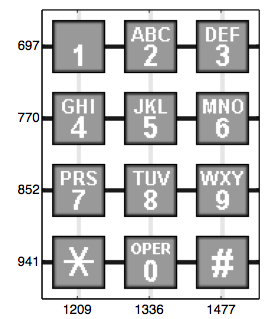
\includegraphics[width=1.5in]{L5-telephonekeypad.png}
%\end{figure} 
%\begin{itemize} 
% \item The basis for touch-tone dialing is the Dual Tone Multi-Frequency. 
%\item When a key is pressed, a tone is generated by superimposing two fundamental tones with different frequency. 
%\end{itemize} 
%} 
%
%\frame{ 
%\frametitle{DFT is used to convert from time-domain to frequency-domain.  } 
%\begin{itemize} 
% \item 
%For example, when $1$ is pressed, the following wave will be observed.
%
%\item Time domain: 
%\begin{figure}
%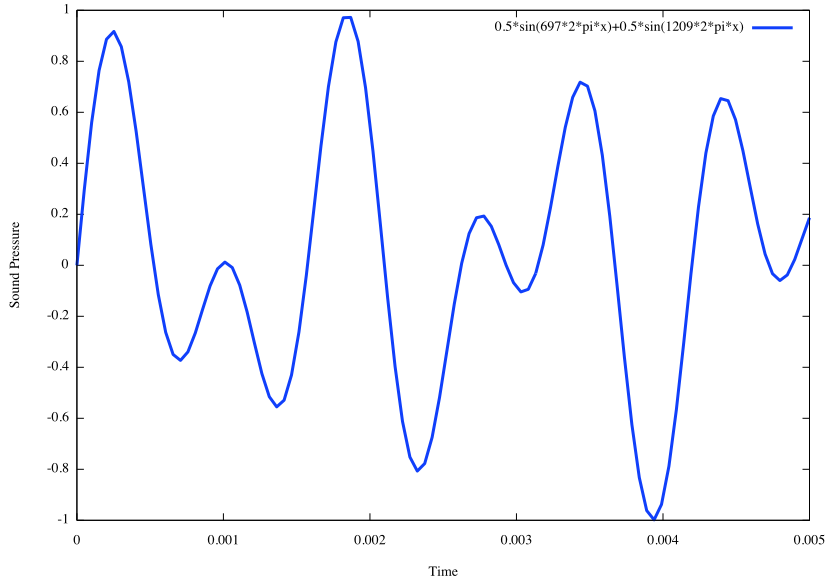
\includegraphics[width=1.3in]{L5-telephonekeypadpress1.png}
%\end{figure} 
%
%\item
%Frequency domain: 
%\begin{figure}
%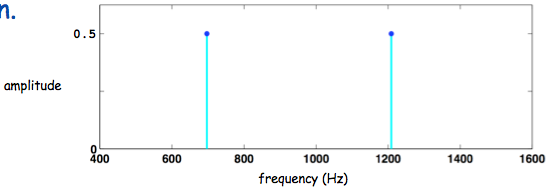
\includegraphics[width=2in]{L5-telephonekeypadpress1fd.png}
%\end{figure} 
%
%\end{itemize} 
%}
%
%
%
%\frame{
%\frametitle{Discrete: acquiring a vector via sampling} 
%
%\begin{itemize}
%\item Sound wave:  
%\begin{figure}
%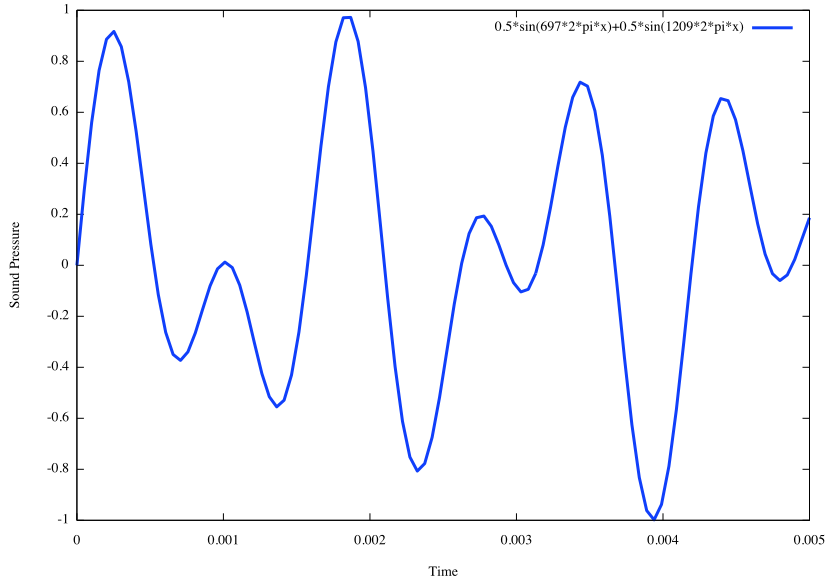
\includegraphics[width=1.5in]{L5-telephonekeypadpress1.png}
%\end{figure} 
%
%\item A vector acquired via sampling: 
%\begin{figure}
%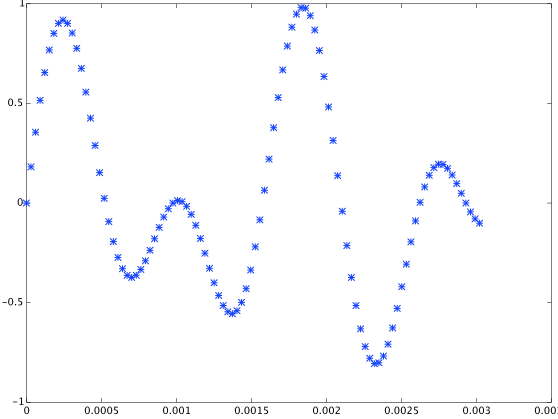
\includegraphics[width=1.5in]{L5-telephonekeypadpress1td.png}
%\end{figure} 
%
%\end{itemize} 
%} 


\frame{
	\frametitle{Outline} 
	\begin{itemize}
		\item DFT: evaluate  a polynomial at $n$ special points; 
		\item FFT: an efficient implementation of DFT; 
		\item Applications of FFT: multiplying two polynomials (and multiplying two $n$-bits integers); time-frequency transform;  solving partial differential equations; 
		\item Appendix: relationship between continuous and discrete Fourier transforms. 
		%why does DFT take this form? 
%	Application: fast multiplication of two polynomials
	\end{itemize}
}

\frame{
\frametitle{DFT: Discrete Fourier Transform } 

\begin{itemize} 
\item DFT evaluates a polynomial $A(x) = a_0 + a_1 x + ... + a_{n-1} x^{n-1}$ at $n$ distinct points $ 1, \omega, \omega^2, ..., \omega^{n-1}$, where  $\omega=e^{\frac{2\pi}{n}i}$ is the $n$-th complex root of unity. 
\item Thus, it transforms the complex vector $a_0, a_1,..., a_{n-1}$  into another complex vector $y_0, y_1, ..., y_{n-1}$, where $y_{k} = A( w^{k})$, i.e., 
\begin{small}
\[
\begin{array}{lllllllllllll}
y_{0} = a_{0}&+\  a_{1}&+\   a_{2} &  \hdots &+\   a_{n-1} \nonumber  \\
y_{1} = a_{0}&+\   a_{1}\omega^{1} &+ \   a_{2}\omega^{2} & \hdots &+\  a_{n-1}\omega^{n-1}  \nonumber \\  
\dots       & \dots   & \dots    &  \hdots & \dots   \nonumber  \\
y_{n-1} = a_{0}&+\   a_{1}\omega^{n-1} &+ \   a_{2}\omega^{2(n-1)} & \hdots &+\  a_{n-1}\omega^{(n-1)^{2}}  
\nonumber 
\end{array}
\]
\end{small}


\item Matrix form: 
\begin{small}
\[
\begin{bmatrix} y_0 \\  y_1 \\ \vdots \\ y_{n-1} \end{bmatrix}  = 
\begin{bmatrix} 1 & 1 & 1 & \dots & 1 \\ 
                          1 & \omega^1 & \omega^2 & \dots & \omega^{n-1} \\ 
                          1 & \omega^2 & \omega^4 & \dots & \omega^{2(n-1)} \\
                          \dots & \dots  & \dots                  & \dots & \dots \\
                          1 & \omega^{n-1} & \omega^{2(n-1)} & \dots & \omega^{(n-1)^2} \end{bmatrix} 
\begin{bmatrix} a_0 \\  a_1 \\ \vdots \\ a_{n-1} \end{bmatrix} 
\] 
\end{small}
\end{itemize} 
} 

\frame{ 
\frametitle{FFT: a fast way to implement DFT [Cooley and Tukey, 1965]} 

\begin{itemize} 
\item Direct matrix-vector multiplication requires $O(n^2)$ operations when using the Horner's method, i.e., \begin{center}
$A(x) = a_{0} + x (a_{1} + x ( a_{2} + \hdots + x a_{n-1}) )$. 
\end{center}
\item FFT: reduce $O(n^2)$ to $O(n\log_2 n)$ using divide-and-conquer  technique. 
\item How does FFT achieve this? Or what calculations are redundant in the direct matrix-vector multiplication approach?
\item Note: The idea of  FFT was proposed by James Cooley and John Tukey in 1965 when analyzing earth-quake data, but the idea can be dated back to F. Gauss. 
\end{itemize}
}

%\frame{
%	\frametitle{Let's evaluate  $A(x)$ at two special points first} 
%
%\begin{itemize}
%	\item Consider evaluating a $7$-degree  polynomial $A(x) = a_0 + a_1 x + a_2 x^2 + ... + a_{7} x^{7}$ at two special points $1, -1$. 
%	\item \textcolor{blue}{\bf Divide: } Break the polynomial into even and odd terms, i.e., 
%		\begin{itemize}
%			\item $A_{even}(x) = a_0 + a_2 x + a_4 x^2 + a_6 x^3 $
%			\item $A_{odd}(x) = a_1  + a_3 x + a_5 x^2 + a_7 x^3 $
%		\end{itemize}
%	 Then we have the following equations: 
%		\begin{itemize}
%			\item $A(x) = A_{even}(x^2) + x A_{odd}(x^2)$ 
%			\item $A(-x) = A_{even}(x^2) - x A_{odd}(x^2)$
%		\end{itemize} 
%	\item\textcolor{blue}{\bf Combine: }  For two special points $1, -1$, we have 
%		\begin{itemize}
%			\item $A(1) = A_{even}(1) +  A_{odd}(1)$ 
%			\item $A(-1) = A_{even}(1) -  A_{odd}(1)$
%		\end{itemize} 
%	\item In other words, the values of $A(x)$ at \textcolor{red}{\bf 2 points $1, -1$} can be calculated based on the values of $A_{even}(x), A_{odd}(x)$ at only \textcolor{red}{\bf  1 point} . 	
%\end{itemize}
%} 	

\frame{
	\frametitle{Let's evaluate  $A(x)$ at four special points } 
%
%\textcolor{blue}{
%	$\min \max_{i} \frac{W_{i}}{E_{i}}$
%}

\begin{itemize}
	\item It is easy to evaluate any $1$-degree polynomial $A(x) = a_0 + a_1 x$ at two  points $1, -1$. 
	Now let's  evaluate  a $3$-degree  polynomial $A(x) = a_0 + a_1 x + a_2 x^2 + a_{3} x^{3}$ at four special points $1, i, -1, -i$. 
	\item \textcolor{blue}{\bf Divide:} Break the polynomial into even and odd terms, i.e., 
		\begin{itemize}
			\item $A_{even}(x) = a_0 + a_2 x  $
			\item $A_{odd}(x) = a_1  + a_3 x  $
		\end{itemize}
	 Then we have the following equations: 
		\begin{itemize}
			\item $A(x) = (a_0 + a_2 x^2) + x(a_1 + a_3 x^2) = A_{even}(x^2) + x A_{odd}(x^2)$ 
			\item $A(-x) = (a_0 + a_2 x^2) - x(a_1 + a_3 x^2) = A_{even}(x^2) - x A_{odd}(x^2)$
		\end{itemize} 
	\item \textcolor{blue}{\bf Combine:} For the 4 special points $1, i, -1, -i$, we have 
		\begin{itemize}
			\item $A(1) = A_{even}(1) +  A_{odd}(1)$ 
			\item $A(i) = A_{even}(-1) + i A_{odd}(-1)$ 
			\item $A(-1) = A_{even}(1) -  A_{odd}(1)$
			\item $A(-i) = A_{even}(-1) - i A_{odd}(-1)$
		\end{itemize} 
	\item In other words, the values of $A(x)$ at \textcolor{red}{\bf  4 points  $1, i, -1, -i$} can be calculated based on the values of $A_{even}(x), A_{odd}(x)$ at \textcolor{red}{\bf  2 points $1, -1$}. 	
\end{itemize}
} 	

\frame{
\frametitle{An example: $n=4$ } 
\begin{small}
\[
\begin{array}{lllllllllllllllllllllllllllll}
y_{0} = a_{0}&+\  a_{1}&+\   a_{2} &+\   a_{3}  \nonumber  \\
y_{1} = a_{0}&+\   a_{1}\omega^{1} &+\   a_{2}\omega^{2} &+\   a_{3}\omega^{3}    \nonumber \\  
y_{2} = a_{0}&+\   a_{1}\omega^{2} &+\   a_{2}\omega^{4} &+\   a_{3}\omega^{6}    \nonumber \\  
y_{3} = a_{0}&+\   a_{1}\omega^{3} &+\   a_{2}\omega^{6} &+\   a_{3}\omega^{9}   \nonumber   
\end{array}
\]
\end{small}
\begin{itemize}
	\item Objective: Evaluate $A(x)$ at 4 points: $1, \omega, \omega^{2},  \omega^{3}$, where $\omega=e^{\frac{1}{4}2\pi i}$. 
\end{itemize}

\begin{figure}
\begin{tikzpicture}[dot/.style={draw,fill=red,circle,inner sep=1pt}]
\def\n{4};
\draw[->] (-1.8,0) -- (2,0) node[below] {$\Re$};f
\draw[->] (0,-1.8) -- (0,2) node[left] {$\Im$};
\draw[help lines] (0,0) circle (1);   
\node[dot] (O) at (0,0) {};
\node[label={above right:${\small +i}$}] (I1) at (0,1) {};
\node[label={below right:${\small -i}$}] (I2) at (0,-1) {};
\node[label={above right:${\small 1}$}] (U1) at (1,0) {};
\node[dot,label={below left:${\small -1}$}] (I2) at (-1,0) {};

\foreach \i in {2,...,\n} {

  \node[dot,label={\i*360/\n-(\i==\n)*45:${\small \omega^{\i}}$}] (w\i) at ( \i*360/\n:1)   {};
   \draw[->] (O) -- (w\i);
  }
  
\foreach \i in {1} {

  \node[dot,label={\i*360/\n-(\i==\n)*45:${\small \omega}$}] (w\i) at ( \i*360/\n:1)   {};
   \draw[->] (O) -- (w\i);
  }
  %\draw[->] (0:.3) arc (0:360/\n:.3);
  %\node at (360/\n/2:.5) {$\alpha$};
  \end{tikzpicture}
\end{figure}


} 

\frame{
\frametitle{Step 1: Simplification  } 
\[
\begin{array}{lllllllllllllllllllllllllllll}
y_{0} = a_{0}&+\  a_{1}&+\   a_{2} &+\   a_{3}&  \nonumber  \\
y_{1} = a_{0}&+\   a_{1}\omega^{1} &+\   a_{2}\omega^{2} &+\   a_{3}\omega^{3}   \nonumber \\  
y_{2} = a_{0}&+\   a_{1}\omega^{2} &+\   a_{2}  &+\   a_{3}\omega^{2}    \nonumber \\  
y_{3} = a_{0}&+\   a_{1}\omega^{3} &+\   a_{2}\omega^{2} &+\   a_{3}\omega^{1}   \nonumber   
 \end{array}
\]
} 


\frame{
\frametitle{Step 2. Divide into odd- and even-terms} 

\[
\begin{array}{lllllllllllllllllllllllllllll}
y_{0} = a_{0}&+\   a_{2} &+\   a_{1}&+\   a_{3} \nonumber  \\
y_{1} = a_{0}&+\   a_{2}\omega^{2} &+\   a_{1}\omega^{1} &+\   a_{3}\omega^{3}  \nonumber \\  
y_{2} = a_{0}&+\   a_{2}   &+\   a_{1}\omega^{2} &+\   a_{3}\omega^{2}   \nonumber \\  
y_{3} = a_{0}&+\   a_{2}\omega^{2} &+\   a_{1}\omega^{3} &+\   a_{3}\omega^{1}    \nonumber  
\end{array}
\]
%The specific order of these terms will be explained later. 
} 




\frame{ 
\frametitle{Key observation: redundant calculations}

%\begin{figure}
%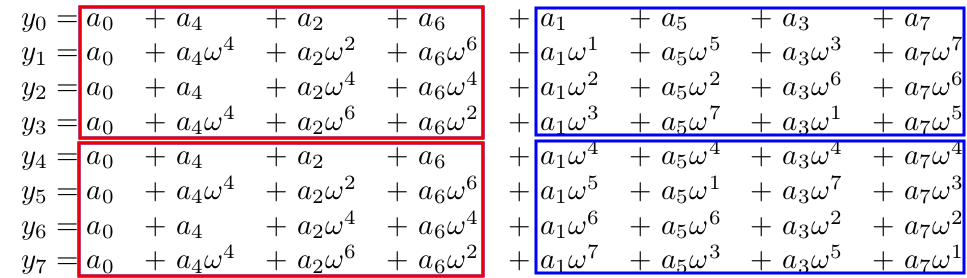
\includegraphics[width=4.6in]{L5-FFT-Step1.png} 
%\end{figure}

\begin{figure}
\begin{tikzpicture}[scale=0.7, auto,swap]

\def\d{0.1};
\draw[thick, red] (-0.05, \d) rectangle (-3.1, 1.6);
\draw[thick, red] (0.05, -\d) rectangle (-3.1, -1.6);

\def\e{0.8};
\draw[thick, blue] (\e, \d) rectangle (4.5, 1.6);
\draw[thick, blue] (\e, -\d) rectangle (4.5, -1.6);

\node at (0,0) {
$
\begin{array}{lllllllllllllllllllllllllllll}
y_{0} = a_{0}&+\   a_{2} &+\   a_{1}&+\   a_{3} \nonumber  \\
y_{1} = a_{0}&+\   a_{2}\omega^{2} &+\   a_{1}\omega^{1} &+\   a_{3}\omega^{3}  \nonumber \\  
y_{2} = a_{0}&+\   a_{2}   &+\   a_{1}\omega^{2} &+\   a_{3}\omega^{2}   \nonumber \\  
y_{3} = a_{0}&+\   a_{2}\omega^{2} &+\   a_{1}\omega^{3} &+\   a_{3}\omega^{1}    \nonumber  
\end{array}
$
 };


\end{tikzpicture}
\end{figure}


Note that the calculations in the two red frames are identical,  and the calculations in the blue frames are also identical after multiplying by $\omega^2$. Here $\omega^2 = -1$ as $\omega = e^{\tfrac{2\pi}{4}i}$.
 
}


\frame{ 
\frametitle{Step 3: Divide-and-conquer }

%\begin{figure}
%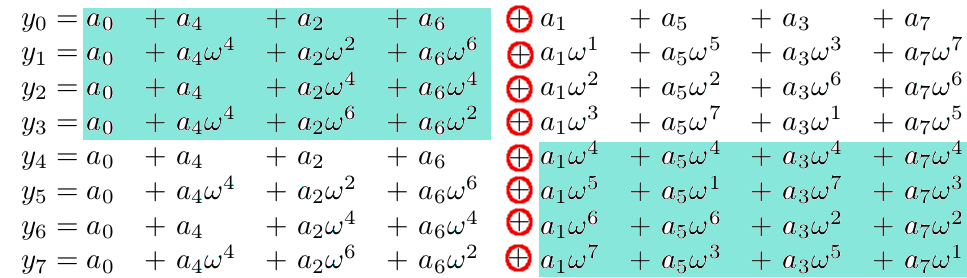
\includegraphics[width=4.6in]{L5-FFT-Step2.png} 
%\end{figure}

\begin{figure}
\begin{tikzpicture}[scale=0.7, auto,swap]

\def\d{0.1};
\draw[green!15, fill=green!15] (-0.05, \d) rectangle (-3.15, 1.6);
%\draw[thick, red] (-\d, -\d) rectangle (-6.7, -2.2);

\def\e{0.8};
%\draw[thick, blue] (\e, \d) rectangle (7.8, 2.2);
\draw[green!15, fill=green!15] (\e, -\d) rectangle (4.5 , -1.6);

\node at (0,0) { 
$
\begin{array}{lllllllllllllllllllllllllllll}
y_{0} = a_{0}&+\   a_{2} &+\   a_{1}&+\   a_{3} \nonumber  \\
y_{1} = a_{0}&+\   a_{2}\omega^{2} &+\   a_{1}\omega^{1} &+\   a_{3}\omega^{3}  \nonumber \\  
y_{2} = a_{0}&+\   a_{2}   &+\   a_{1}\omega^{2} &+\   a_{3}\omega^{2}   \nonumber \\  
y_{3} = a_{0}&+\   a_{2}\omega^{2} &+\   a_{1}\omega^{3} &+\   a_{3}\omega^{1}    \nonumber  
\end{array}
$
 };


\end{tikzpicture}
\end{figure}

Thus the calculations in the top-left and  bottom-right frames are redundant. We need only $2+4+2=4\times \log_{2} 4$ calculations.

}  



\frame{
\frametitle{Another example: $n=8$ } 
\begin{footnotesize}
\[
\begin{array}{lllllllllllllllllllllllllllll}
y_{0} = a_{0}&+\  a_{1}&+\   a_{2} &+\   a_{3}&+\   a_{4}&+\  a_{5}&+\  a_{6}&+\   a_{7} \nonumber  \\
y_{1} = a_{0}&+\   a_{1}\omega^{1} &+\   a_{2}\omega^{2} &+\   a_{3}\omega^{3} &+\  a_{4}\omega^{4} &+\  a_{5}\omega^{5} &+\   a_{6}\omega^{6} &+\  a_{7}\omega^{7}  \nonumber \\  
y_{2} = a_{0}&+\   a_{1}\omega^{2} &+\   a_{2}\omega^{4} &+\   a_{3}\omega^{6} &+\  a_{4}\omega^{8} &+\  a_{5}\omega^{10} &+\   a_{6}\omega^{12} &+\  a_{7}\omega^{14}  \nonumber \\  
y_{3} = a_{0}&+\   a_{1}\omega^{3} &+\   a_{2}\omega^{6} &+\   a_{3}\omega^{9} &+\  a_{4}\omega^{12} &+\  a_{5}\omega^{15} &+\   a_{6}\omega^{18} &+\  a_{7}\omega^{21}  \nonumber \\  
y_{4} = a_{0}&+\  a_{1}\omega^{4} &+\   a_{2} &+\   a_{3}\omega^{12} &+\  
a_{4}\omega^{16} &+\  a_{5}\omega^{20} &+\  a_{6}\omega^{24} &+\  
a_{7}\omega^{28}  \nonumber \\  
y_{5} = a_{0}&+\   a_{1}\omega^{5} &+\   a_{2}\omega^{10} &+\   a_{3}\omega^{15} &+\  a_{4}\omega^{20} &+\  a_{5}\omega^{25} &+\   a_{6}\omega^{30} &+\  a_{7}\omega^{35}  \nonumber \\  
y_{6} = a_{0}&+\   a_{1}\omega^{6} &+\   a_{2}\omega^{12} &+\   a_{3}\omega^{18} &+\  a_{4}\omega^{24} &+\  a_{5}\omega^{30} &+\   a_{6}\omega^{36} &+\  a_{7}\omega^{42}  \nonumber \\  
y_{7} = a_{0}&+\   a_{1}\omega^{7} &+\   a_{2}\omega^{14} &+\   a_{3}\omega^{21} &+\  a_{4}\omega^{28} &+\  a_{5}\omega^{35} &+\   a_{6}\omega^{42} &+\  a_{7}\omega^{49}  \nonumber 
\end{array}
\]
\end{footnotesize}
\begin{itemize}
	\item Objective: Evaluate $A(x)$ at 8 points: $1, \omega, \omega^{2}, ..., \omega^{7}$, where $\omega=e^{\frac{1}{8}2\pi i}$. 
\end{itemize}

\begin{figure}
\begin{tikzpicture}[dot/.style={draw,fill=red,circle,inner sep=1pt}]
\def\n{8};
\draw[->] (-1.8,0) -- (2,0) node[below] {$\Re$};f
\draw[->] (0,-1.8) -- (0,2) node[left] {$\Im$};
\draw[help lines] (0,0) circle (1);   
\node[dot] (O) at (0,0) {};
\node[label={above right:${\small +i}$}] (I1) at (0,1) {};
\node[label={below right:${\small -i}$}] (I2) at (0,-1) {};
\node[label={above right:${\small 1}$}] (U1) at (1,0) {};
\node[dot,label={below left:${\small -1}$}] (I2) at (-1,0) {};

\foreach \i in {1,...,\n} {

  \node[dot,label={\i*360/\n-(\i==\n)*45:${\small \omega^{\i}}$}] (w\i) at ( \i*360/\n:1)   {};
   \draw[->] (O) -- (w\i);
  }
  %\draw[->] (0:.3) arc (0:360/\n:.3);
  %\node at (360/\n/2:.5) {$\alpha$};
  \end{tikzpicture}
\end{figure}


} 

\frame{
\frametitle{Step 1: Simplification  } 
\begin{small}
\[
\begin{array}{lllllllllllllllllllllllllllll}
y_{0} = a_{0}&+\  a_{1}&+\   a_{2} &+\   a_{3}&+\   a_{4}&+\  a_{5}&+\  a_{6}&+\   a_{7} \nonumber  \\
y_{1} = a_{0}&+\   a_{1}\omega^{1} &+\   a_{2}\omega^{2} &+\   a_{3}\omega^{3} &+\  a_{4}\omega^{4} &+\  a_{5}\omega^{5} &+\   a_{6}\omega^{6} &+\  a_{7}\omega^{7}  \nonumber \\  
y_{2} = a_{0}&+\   a_{1}\omega^{2} &+\   a_{2}\omega^{4} &+\   a_{3}\omega^{6} &+\  a_{4} &+\  a_{5}\omega^{2} &+\   a_{6}\omega^{4} &+\  a_{7}\omega^{6}  \nonumber \\  
y_{3} = a_{0}&+\   a_{1}\omega^{3} &+\   a_{2}\omega^{6} &+\   a_{3}\omega^{1} &+\  a_{4}\omega^{4} &+\  a_{5}\omega^{7} &+\   a_{6}\omega^{2} &+\  a_{7}\omega^{5}  \nonumber \\  
y_{4} = a_{0}&+\  a_{1}\omega^{4} &+\   a_{2}\omega^{8} &+\   a_{3}\omega^{4} &+\   a_{4} &+\  a_{5}\omega^{4} &+\  a_{6} &+\   a_{7}\omega^{4}  \nonumber \\  
y_{5} = a_{0}&+\   a_{1}\omega^{5} &+\   a_{2}\omega^{2} &+\   a_{3}\omega^{7} &+\  a_{4}\omega^{4} &+\  a_{5}\omega^{1} &+\   a_{6}\omega^{6} &+\  a_{7}\omega^{3}  \nonumber \\  
y_{6} = a_{0}&+\   a_{1}\omega^{6} &+\   a_{2}\omega^{4} &+\   a_{3}\omega^{2} &+\  a_{4} &+\  a_{5}\omega^{6} &+\   a_{6}\omega^{4} &+\  a_{7}\omega^{2}  \nonumber \\  
y_{7} = a_{0}&+\   a_{1}\omega^{7} &+\   a_{2}\omega^{6} &+\   a_{3}\omega^{5} &+\  a_{4}\omega^{4} &+\  a_{5}\omega^{3} &+\   a_{6}\omega^{2} &+\  a_{7}\omega^{1}  \nonumber 
\end{array}
\]
\end{small}
} 


\frame{
\frametitle{Step 2. Divide into odd- and even-terms} 
\begin{small}
\[
\begin{array}{lllllllllllllllllllllllllllll}
y_{0} = a_{0}&+\   a_{4} &+\   a_{2}&+\   a_{6}&+\  a_{1}&+\  a_{5}&+\   a_{3}&+\  a_{7} \nonumber  \\
y_{1} = a_{0}&+\   a_{4}\omega^{4} &+\   a_{2}\omega^{2} &+\   a_{6}\omega^{6} &+\  a_{1}\omega^{1} &+\  a_{5}\omega^{5} &+\   a_{3}\omega^{3} &+\  a_{7}\omega^{7}  \nonumber \\  
y_{2} = a_{0}&+\   a_{4} &+\   a_{2}\omega^{4} &+\   a_{6}\omega^{4} &+\  a_{1}\omega^{2} &+\  a_{5}\omega^{2} &+\   a_{3}\omega^{6} &+\  a_{7}\omega^{6}  \nonumber \\  
y_{3} = a_{0}&+\   a_{4}\omega^{4} &+\   a_{2}\omega^{6} &+\   a_{6}\omega^{2}
&+\  a_{1}\omega^{3} &+\  a_{5}\omega^{7} &+\   a_{3}\omega^{1} &+\ 
a_{7}\omega^{5}  \nonumber \\  
y_{4} = a_{0}&+\   a_{4} &+\   a_{2} &+\   a_{6} &+\  a_{1}\omega^{4} &+\  a_{5}\omega^{4} &+\   a_{3}\omega^{4} &+\  a_{7}\omega^{4}  \nonumber \\  
y_{5} = a_{0}&+\   a_{4}\omega^{4} &+\   a_{2}\omega^{2} &+\   a_{6}\omega^{6} &+\  a_{1}\omega^{5} &+\  a_{5}\omega^{1} &+\   a_{3}\omega^{7} &+\  a_{7}\omega^{3}  \nonumber \\  
y_{6} = a_{0}&+\   a_{4} &+\   a_{2}\omega^{4} &+\   a_{6}\omega^{4} &+\  a_{1}\omega^{6} &+\  a_{5}\omega^{6} &+\   a_{3}\omega^{2} &+\  a_{7}\omega^{2}  \nonumber \\  
y_{7} = a_{0}&+\   a_{4}\omega^{4} &+\   a_{2}\omega^{6} &+\   a_{6}\omega^{2} &+\  a_{1}\omega^{7} &+\  a_{5}\omega^{3} &+\   a_{3}\omega^{5} &+\  a_{7}\omega^{1}  \nonumber 
\end{array}
\]
\end{small}
The specific order of these terms will be explained later. 
} 




\frame{ 
\frametitle{Key observation: redundant calculations}

%\begin{figure}
%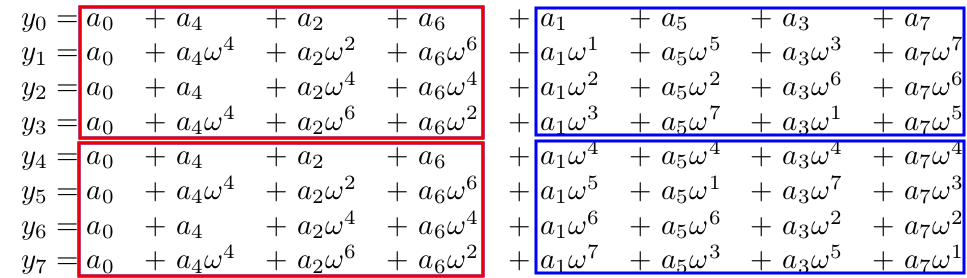
\includegraphics[width=4.6in]{L5-FFT-Step1.png} 
%\end{figure}

\begin{figure}
\begin{tikzpicture}[scale=0.7, auto,swap]

\def\d{0.1};
\draw[thick, red] (-\d, \d) rectangle (-6.7, 2.2);
\draw[thick, red] (-\d, -\d) rectangle (-6.7, -2.2);

\def\e{0.68};
\draw[thick, blue] (\e, \d) rectangle (7.8, 2.2);
\draw[thick, blue] (\e, -\d) rectangle (7.8, -2.2);

\node at (0,0) {\begin{footnotesize}
$
\begin{array}{lllllllllllllllllllllllllllll}
y_{0} = a_{0}&+\   a_{4} &+\   a_{2}&+\   a_{6}&+\  a_{1}&+\  a_{5}&+\   a_{3}&+\  a_{7} \nonumber  \\
y_{1} = a_{0}&+\   a_{4}\omega^{4} &+\   a_{2}\omega^{2} &+\   a_{6}\omega^{6} &+\  a_{1}\omega^{1} &+\  a_{5}\omega^{5} &+\   a_{3}\omega^{3} &+\  a_{7}\omega^{7}  \nonumber \\  
y_{2} = a_{0}&+\   a_{4} &+\   a_{2}\omega^{4} &+\   a_{6}\omega^{4} &+\  a_{1}\omega^{2} &+\  a_{5}\omega^{2} &+\   a_{3}\omega^{6} &+\  a_{7}\omega^{6}  \nonumber \\  
y_{3} = a_{0}&+\   a_{4}\omega^{4} &+\   a_{2}\omega^{6} &+\   a_{6}\omega^{2}
&+\  a_{1}\omega^{3} &+\  a_{5}\omega^{7} &+\   a_{3}\omega^{1} &+\ 
a_{7}\omega^{5}  \nonumber \\  
y_{4} = a_{0}&+\   a_{4} &+\   a_{2} &+\   a_{6} &+\  a_{1}\omega^{4} &+\  a_{5}\omega^{4} &+\   a_{3}\omega^{4} &+\  a_{7}\omega^{4}  \nonumber \\  
y_{5} = a_{0}&+\   a_{4}\omega^{4} &+\   a_{2}\omega^{2} &+\   a_{6}\omega^{6} &+\  a_{1}\omega^{5} &+\  a_{5}\omega^{1} &+\   a_{3}\omega^{7} &+\  a_{7}\omega^{3}  \nonumber \\  
y_{6} = a_{0}&+\   a_{4} &+\   a_{2}\omega^{4} &+\   a_{6}\omega^{4} &+\  a_{1}\omega^{6} &+\  a_{5}\omega^{6} &+\   a_{3}\omega^{2} &+\  a_{7}\omega^{2}  \nonumber \\  
y_{7} = a_{0}&+\   a_{4}\omega^{4} &+\   a_{2}\omega^{6} &+\   a_{6}\omega^{2} &+\  a_{1}\omega^{7} &+\  a_{5}\omega^{3} &+\   a_{3}\omega^{5} &+\  a_{7}\omega^{1}  \nonumber 
\end{array}
$
\end{footnotesize} };


\end{tikzpicture}
\end{figure}


Note that the calculations in the two red frames are identical, and the  calculations in the blue frames are also identical after multiplying by $\omega^4$. Here $\omega^4 = -1$ as $\omega = e^{\tfrac{2\pi}{8}i}$.
 
}


\frame{ 
\frametitle{Step 3: Divide-and-conquer }

%\begin{figure}
%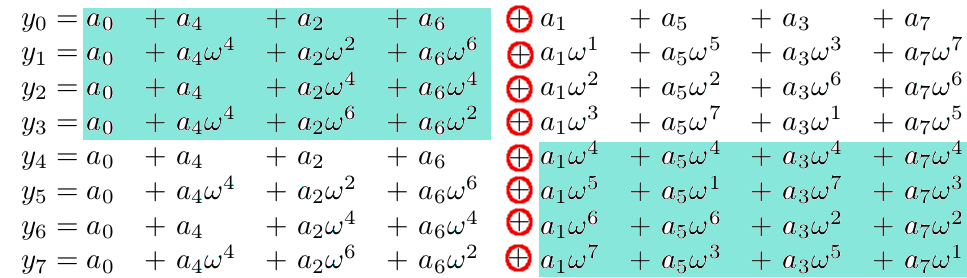
\includegraphics[width=4.6in]{L5-FFT-Step2.png} 
%\end{figure}

\begin{figure}
\begin{tikzpicture}[scale=0.7, auto,swap]

\def\d{0.1};
\draw[green!15, fill=green!15] (-\d, \d) rectangle (-6.7, 2.2);
%\draw[thick, red] (-\d, -\d) rectangle (-6.7, -2.2);

\def\e{0.68};
%\draw[thick, blue] (\e, \d) rectangle (7.8, 2.2);
\draw[green!15, fill=green!15] (\e, -\d) rectangle (7.8, -2.2);

\node at (0,0) {\begin{footnotesize}
$
\begin{array}{lllllllllllllllllllllllllllll}
y_{0} = a_{0}&+\   a_{4} &+\   a_{2}&+\   a_{6}&+\  a_{1}&+\  a_{5}&+\   a_{3}&+\  a_{7} \nonumber  \\
y_{1} = a_{0}&+\   a_{4}\omega^{4} &+\   a_{2}\omega^{2} &+\   a_{6}\omega^{6} &+\  a_{1}\omega^{1} &+\  a_{5}\omega^{5} &+\   a_{3}\omega^{3} &+\  a_{7}\omega^{7}  \nonumber \\  
y_{2} = a_{0}&+\   a_{4} &+\   a_{2}\omega^{4} &+\   a_{6}\omega^{4} &+\  a_{1}\omega^{2} &+\  a_{5}\omega^{2} &+\   a_{3}\omega^{6} &+\  a_{7}\omega^{6}  \nonumber \\  
y_{3} = a_{0}&+\   a_{4}\omega^{4} &+\   a_{2}\omega^{6} &+\   a_{6}\omega^{2}
&+\  a_{1}\omega^{3} &+\  a_{5}\omega^{7} &+\   a_{3}\omega^{1} &+\ 
a_{7}\omega^{5}  \nonumber \\  
y_{4} = a_{0}&+\   a_{4} &+\   a_{2} &+\   a_{6} &+\  a_{1}\omega^{4} &+\  a_{5}\omega^{4} &+\   a_{3}\omega^{4} &+\  a_{7}\omega^{4}  \nonumber \\  
y_{5} = a_{0}&+\   a_{4}\omega^{4} &+\   a_{2}\omega^{2} &+\   a_{6}\omega^{6} &+\  a_{1}\omega^{5} &+\  a_{5}\omega^{1} &+\   a_{3}\omega^{7} &+\  a_{7}\omega^{3}  \nonumber \\  
y_{6} = a_{0}&+\   a_{4} &+\   a_{2}\omega^{4} &+\   a_{6}\omega^{4} &+\  a_{1}\omega^{6} &+\  a_{5}\omega^{6} &+\   a_{3}\omega^{2} &+\  a_{7}\omega^{2}  \nonumber \\  
y_{7} = a_{0}&+\   a_{4}\omega^{4} &+\   a_{2}\omega^{6} &+\   a_{6}\omega^{2} &+\  a_{1}\omega^{7} &+\  a_{5}\omega^{3} &+\   a_{3}\omega^{5} &+\  a_{7}\omega^{1}  \nonumber 
\end{array}
$
\end{footnotesize} };


\end{tikzpicture}
\end{figure}

Thus the calculations in the top-left and  bottom-right frames are redundant. 
}  


\frame{ 
\frametitle{Step 3: Divide-and-conquer }


\begin{figure}
\begin{tikzpicture}[scale=0.7, auto,swap]

\def\d{0.1};
\draw[green!15, fill=green!15] (-\d, \d) rectangle (-6.7, 2.2);
%\draw[thick, red] (-\d, -\d) rectangle (-6.7, -2.2);
\draw[green!15, fill=green!15] (-6.7, -\d) rectangle (-4, -1.1);
\draw[green!15, fill=green!15] (-3.2, -1.1) rectangle (-\d, -2.2);



\def\e{0.68};
%\draw[thick, blue] (\e, \d) rectangle (7.8, 2.2);
\draw[green!15, fill=green!15] (\e, -\d) rectangle (7.8, -2.2);
\draw[green!15, fill=green!15] (\e, 2.2) rectangle (3.8, 1.1);
\draw[green!15, fill=green!15] (4.7, 1.1) rectangle (7.8, \d);


\node at (0,0) {\begin{footnotesize}
$
\begin{array}{lllllllllllllllllllllllllllll}
y_{0} = a_{0}&+\   a_{4} &+\   a_{2}&+\   a_{6}&+\  a_{1}&+\  a_{5}&+\   a_{3}&+\  a_{7} \nonumber  \\
y_{1} = a_{0}&+\   a_{4}\omega^{4} &+\   a_{2}\omega^{2} &+\   a_{6}\omega^{6} &+\  a_{1}\omega^{1} &+\  a_{5}\omega^{5} &+\   a_{3}\omega^{3} &+\  a_{7}\omega^{7}  \nonumber \\  
y_{2} = a_{0}&+\   a_{4} &+\   a_{2}\omega^{4} &+\   a_{6}\omega^{4} &+\  a_{1}\omega^{2} &+\  a_{5}\omega^{2} &+\   a_{3}\omega^{6} &+\  a_{7}\omega^{6}  \nonumber \\  
y_{3} = a_{0}&+\   a_{4}\omega^{4} &+\   a_{2}\omega^{6} &+\   a_{6}\omega^{2}
&+\  a_{1}\omega^{3} &+\  a_{5}\omega^{7} &+\   a_{3}\omega^{1} &+\ 
a_{7}\omega^{5}  \nonumber \\  
y_{4} = a_{0}&+\   a_{4} &+\   a_{2} &+\   a_{6} &+\  a_{1}\omega^{4} &+\  a_{5}\omega^{4} &+\   a_{3}\omega^{4} &+\  a_{7}\omega^{4}  \nonumber \\  
y_{5} = a_{0}&+\   a_{4}\omega^{4} &+\   a_{2}\omega^{2} &+\   a_{6}\omega^{6} &+\  a_{1}\omega^{5} &+\  a_{5}\omega^{1} &+\   a_{3}\omega^{7} &+\  a_{7}\omega^{3}  \nonumber \\  
y_{6} = a_{0}&+\   a_{4} &+\   a_{2}\omega^{4} &+\   a_{6}\omega^{4} &+\  a_{1}\omega^{6} &+\  a_{5}\omega^{6} &+\   a_{3}\omega^{2} &+\  a_{7}\omega^{2}  \nonumber \\  
y_{7} = a_{0}&+\   a_{4}\omega^{4} &+\   a_{2}\omega^{6} &+\   a_{6}\omega^{2} &+\  a_{1}\omega^{7} &+\  a_{5}\omega^{3} &+\   a_{3}\omega^{5} &+\  a_{7}\omega^{1}  \nonumber 
\end{array}
$
\end{footnotesize} };


\end{tikzpicture}
\end{figure}
%\begin{figure}
%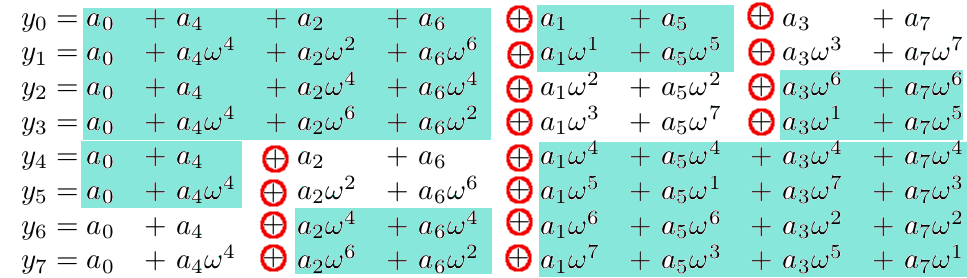
\includegraphics[width=4.6in]{L5-FFT-Step3.png} 
%\end{figure}
Finally, we need only $2+4+2+8+2+4+2=8\times \log_{2} 8$ calculations.

}  

%\frame{ 
%\frametitle{Step 3: divide-and-conquer }
%
%%\begin{figure}
%%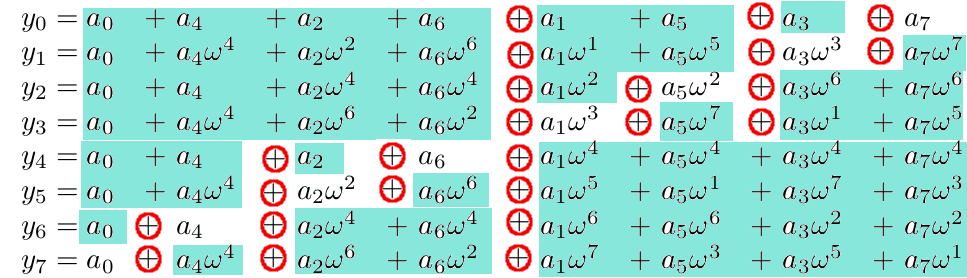
\includegraphics[width=4.6in]{L5-FFT-Step4.png} 
%%\end{figure}
%
%
%\begin{figure}
%\begin{tikzpicture}[scale=0.7, auto,swap]
%
%\def\d{0.1};
%\draw[green!15, fill=green!15] (-\d, \d) rectangle (-6.7, 2.2);
%%\draw[thick, red] (-\d, -\d) rectangle (-6.7, -2.2);
%
%\def\e{0.68};
%%\draw[thick, blue] (\e, \d) rectangle (7.8, 2.2);
%\draw[green!15, fill=green!15] (\e, -\d) rectangle (7.8, -2.2);
%
%\node at (0,0) {\begin{footnotesize}
%$
%\begin{array}{lllllllllllllllllllllllllllll}
%y_{0} = a_{0}&+\   a_{4} &+\   a_{2}&+\   a_{6}&+\  a_{1}&+\  a_{5}&+\   a_{3}&+\  a_{7} \nonumber  \\
%y_{1} = a_{0}&+\   a_{4}\omega^{4} &+\   a_{2}\omega^{2} &+\   a_{6}\omega^{6} &+\  a_{1}\omega^{1} &+\  a_{5}\omega^{5} &+\   a_{3}\omega^{3} &+\  a_{7}\omega^{7}  \nonumber \\  
%y_{2} = a_{0}&+\   a_{4} &+\   a_{2}\omega^{4} &+\   a_{6}\omega^{4} &+\  a_{1}\omega^{2} &+\  a_{5}\omega^{2} &+\   a_{3}\omega^{6} &+\  a_{7}\omega^{6}  \nonumber \\  
%y_{3} = a_{0}&+\   a_{4}\omega^{4} &+\   a_{2}\omega^{6} &+\   a_{6}\omega^{2}
%&+\  a_{1}\omega^{3} &+\  a_{5}\omega^{7} &+\   a_{3}\omega^{1} &+\ 
%a_{7}\omega^{5}  \nonumber \\  
%y_{4} = a_{0}&+\   a_{4} &+\   a_{2} &+\   a_{6} &+\  a_{1}\omega^{4} &+\  a_{5}\omega^{4} &+\   a_{3}\omega^{4} &+\  a_{7}\omega^{4}  \nonumber \\  
%y_{5} = a_{0}&+\   a_{4}\omega^{4} &+\   a_{2}\omega^{2} &+\   a_{6}\omega^{6} &+\  a_{1}\omega^{5} &+\  a_{5}\omega^{1} &+\   a_{3}\omega^{7} &+\  a_{7}\omega^{3}  \nonumber \\  
%y_{6} = a_{0}&+\   a_{4} &+\   a_{2}\omega^{4} &+\   a_{6}\omega^{4} &+\  a_{1}\omega^{6} &+\  a_{5}\omega^{6} &+\   a_{3}\omega^{2} &+\  a_{7}\omega^{2}  \nonumber \\  
%y_{7} = a_{0}&+\   a_{4}\omega^{4} &+\   a_{2}\omega^{6} &+\   a_{6}\omega^{2} &+\  a_{1}\omega^{7} &+\  a_{5}\omega^{3} &+\   a_{3}\omega^{5} &+\  a_{7}\omega^{1}  \nonumber 
%\end{array}
%$
%\end{footnotesize} };
%
%
%\end{tikzpicture}
%\end{figure}
%Finally, we need $8\times \log(8)$ calculations.
%}  

\frame{ 
\frametitle{The final order } 
%\begin{figure}
%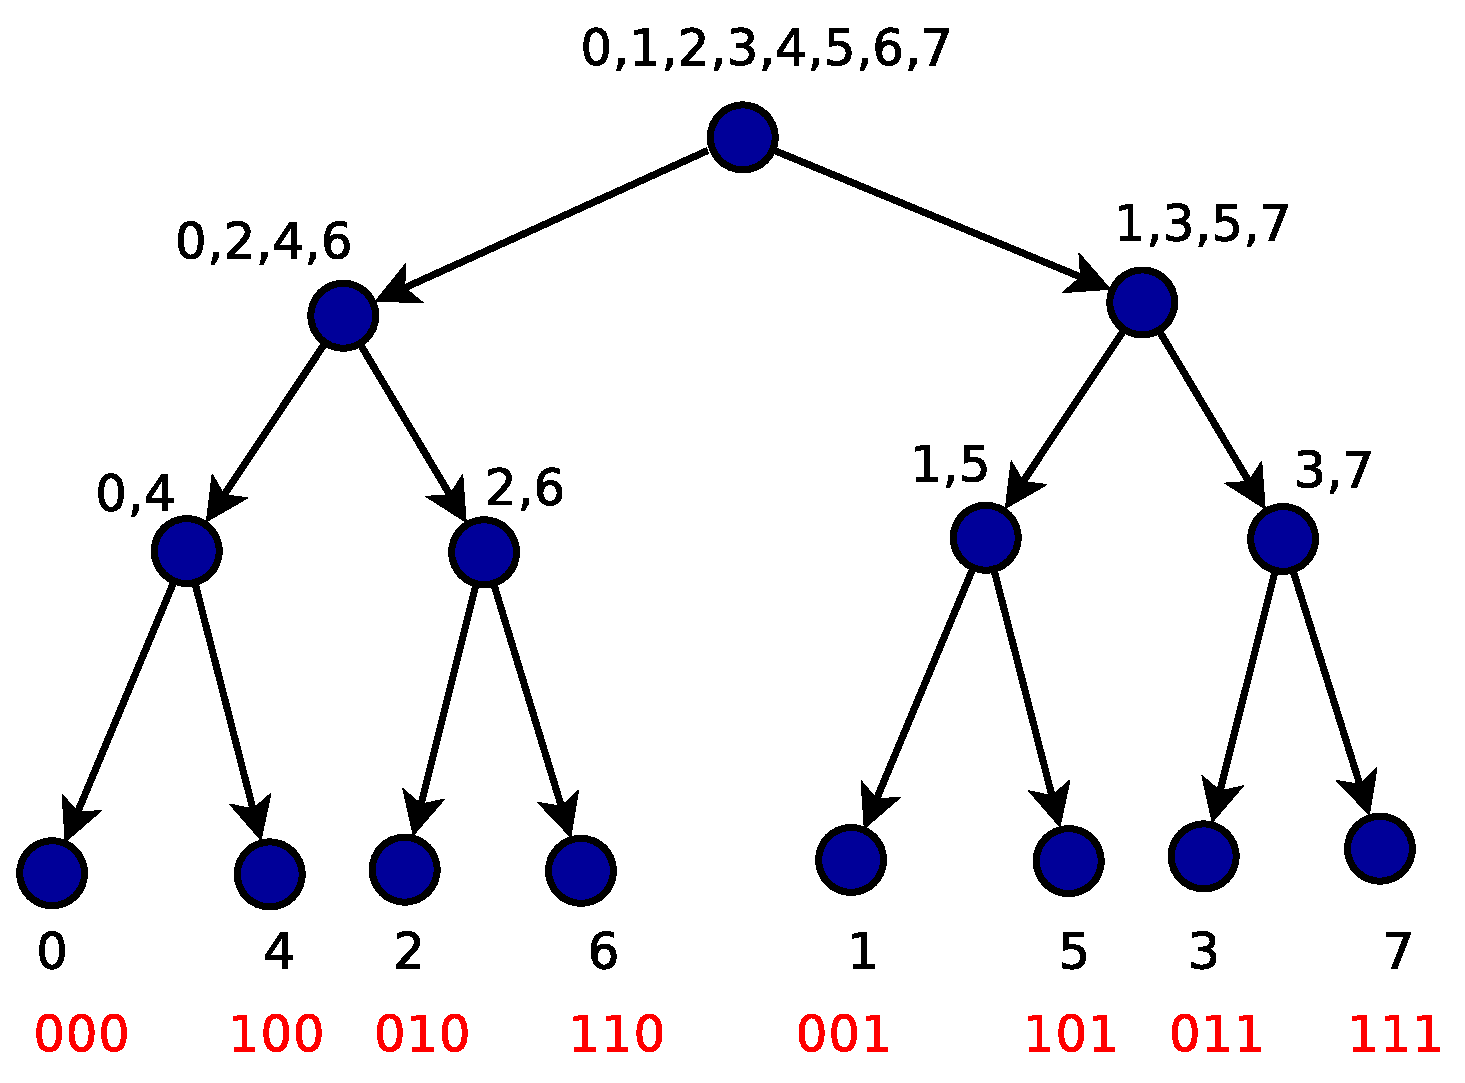
\includegraphics[width=4.in]{L5-FFT-tree.eps} 
%\end{figure}

\begin{figure}
\begin{tikzpicture}[scale=1., auto,swap]
    % Draw a 7,11 network
    % First we draw the vertices
    \foreach \pos/\name/\label in {{(0,0)/root/6}, 
    {(-3,-1)/L/10}, {(3,-1)/R/8}, 
    {(-4.5,-2)/LL/12}, {(-1.5, -2)/LR/18}, {(1.5, -2)/RL/11}, {(4.5, -2)/RR/25}, 
    {(-5.2, -3)/LLL/21}, {(-3.8, -3)/LLR/17},{(-2.2, -3)/LRL/21}, {(-0.8, -3)/LRR/17},
    {(5.2, -3)/RRR/21}, {(3.8, -3)/RRL/17},{(2.2, -3)/RLR/21}, {(0.8, -3)/RLL/17}}
        \node[smallvertex,draw=black, fill=blue!20] (\name) at \pos { };
  
    % Connect vertices with edges and draw weights
  \foreach \source/ \dest /\weight in {root/L/{}, root/R/{}, L/LL/{}, L/LR/{}, R/RL/{}, R/RR/{}, LL/LLL/{}, LL/LLR/{},LR/LRL/{},LR/LRR/{}, RL/RLL/{}, RL/RLR/{}, RR/RRL/{}, RR/RRR/{}}
        \path[undirectededge] (\source) -- node[weight] {$\weight$} (\dest);
%       \draw[dashed, ->] (0,0) arc  (120:60:2);
 
 \node[above] at (0, 0.2) {\tiny $0, 1, 2, 3, 4, 5, 6, 7$}; 
 \node at (-4, -1)  {\tiny $0, 2, 4, 6$};
 \node at (4, -1)  {\tiny $1, 3, 5, 7$};
 
\node at (-5, -2)  {\tiny $0, 4$};
\node at (-1, -2)  {\tiny $2, 6$};
 \node at (5, -2)  {\tiny $3, 7$};
 \node at (1, -2)  {\tiny $1, 5$};

 \node at (-5.2, -3.3)  {\tiny $0$};
 \node at (-3.8, -3.3)  {\tiny $4$};
 \node at (-2.2, -3.3)  {\tiny $2$};
 \node at (-0.8, -3.3)  {\tiny $6$};
 \node at (0.8, -3.3)  {\tiny $1$};
 \node at (2.2, -3.3)  {\tiny $5$};
 \node at (3.8, -3.3)  {\tiny $3$};
 \node at (5.2, -3.3)  {\tiny $7$};

 \node[red] at (-5.2, -3.6)  {\tiny $000$};
 \node[red] at (-3.8, -3.6)  {\tiny $100$};
 \node[red] at (-2.2, -3.6)  {\tiny $010$};
 \node[red] at (-0.8, -3.6)  {\tiny $110$};
 \node[red] at (0.8, -3.6)  {\tiny $001$};
 \node[red] at (2.2, -3.6)  {\tiny $101$};
 \node[red] at (3.8, -3.6)  {\tiny $011$};
 \node[red] at (5.2, -3.6)  {\tiny $111$};


 
   \end{tikzpicture}
\end{figure}


} 



\frame{
\frametitle{FFT Algorithm } 

{\sc FFT}$( n, a_0, a_1, ... , a_{n-1} )$  
\begin{algorithmic}[1]
\IF{$n == 1 $}
	\RETURN{ $a_0$ }; 
\ENDIF
\STATE{$(E_0, E_1,..., E_{\frac{n}{2} - 1} ) =${\sc FFT}$( \frac{n}{2}, a_0, a_2, ..., a_{n-2} );$ }
\STATE{$(O_0, O_1,..., O_{\frac{n}{2} - 1} ) = $ {\sc FFT}$( \frac{n}{2}, a_1, a_3, ..., a_{n - 1 }); $}  
\FOR{$k=0$ to $\frac{n}{2} - 1$ } 
	\STATE{$ \omega^{k}  = e^{ \frac{2 \pi }{n} k i  }$; }
	\STATE{$y_k = E_k + \omega^k  O_k$; } 
	\STATE{$y_{\frac{n}{2}+ k} = E_k - \omega^k  O_k$; } 
\ENDFOR
\RETURN{$(y_0, y_1, ..., y_{n-1} )$};
\end{algorithmic} 
\begin{itemize}
	\item Here {\sc FFT}$( \frac{n}{2}, a_0, a_2, ..., a_{n} )$ computes the polynomial $A_{even}(x) = a_0 + a_2 x + ... + a_n x^{\tfrac{n}{2}}$ at $\frac{n}{2}$ points $1, \omega^2, \omega^4, ...,  \omega^{n-2}$, and {\sc FFT}$( \frac{n}{2}, a_1, a_3, ..., a_{n - 1})$ computes the polynomial $A_{odd}(x) = a_1 + a_3 x + ... + a_{n-1} x^{\tfrac{n}{2}}$ at these points. 
\end{itemize}

} 





\frame{
\frametitle{Inverse Discrete Fourier Transform } 

\begin{itemize} 
\item Inverse Discrete Fourier Transform: to determine coefficients of a polynomial  $a_0, a_1, ..., a_{n-1}$ based on $n$ point-value pairs $(1, y_0), (\omega, y_1), ..., (\omega^{n-1}, y_{n-1})$, where 
$y_{k} = A(\omega^{k})$,  and $A(x) = a_{0} + a_{1} x + a_{2}x^{2}+...+a_{n-1}x^{n-1}$.  

\item Matrix form
\[
\begin{bmatrix} y_0 \\  y_1 \\ \vdots \\ y_{n-1} \end{bmatrix}  = 
\begin{bmatrix} 1 & 1 & 1 & \dots & 1 \\ 
                          1 & \omega^1 & \omega^2 & \dots & \omega^{n-1} \\ 
                          1 & \omega^2 & \omega^4 & \dots & \omega^{2(n-1)} \\
                          \dots & \dots  & \dots                  & \dots & \dots \\
                          1 & \omega^{n-1} & \omega^{2(n-1)} & \dots & \omega^{(n-1)^2} \end{bmatrix} 
\begin{bmatrix} a_0 \\  a_1 \\ \vdots \\ a_{n-1} \end{bmatrix} 
\] 
\item It takes $O(n^{3})$ to calculate the inverse matrix when using the Gaussian elimination technique. 
\end{itemize} 
} 

\frame{
\frametitle{Inverse Discrete Fourier Transform  cont'd} 
\begin{itemize} 
\item Matrix form
\[
\begin{bmatrix} a_0 \\  a_1 \\ \vdots \\ a_{n-1} \end{bmatrix}  = \frac{1}{n}
\begin{bmatrix} 1 & 1 & 1 & \dots & 1 \\ 
                          1 & \bar{ \omega}^1 & \bar{ \omega}^2 & \dots & \bar{\omega}^{n-1} \\ 
                          1 & \bar{\omega}^2 & \bar{\omega}^4 & \dots & \bar{\omega}^{2(n-1)} \\
                          \dots & \dots  & \dots                  & \dots & \dots \\
                          1 & \bar{\omega}^{n-1} & \bar{\omega}^{2(n-1)} & \dots & \bar{\omega}^{(n-1)^2} \end{bmatrix} 
\begin{bmatrix} y_0 \\  y_1 \\ \vdots \\ y_{n-1} \end{bmatrix} 
\] 
\item Reason: it turns out that  it is nearly its own inverse. More precisely, the conjugate transpose of this matrix is its own inverse. 
\end{itemize} 
}

\frame{
\frametitle{IFFT Algorithm } 

{\sc IFFT}$( n, y_0, y_1, ... , y_{n-1} )$  
\begin{algorithmic}[1]
\IF{$n == 1 $}
	\RETURN{$y_0$ }; 
\ENDIF
\STATE{$(E_0, E_1,..., E_{\frac{n}{2} - 1} ) =$ {\sc IFFT}$( \frac{n}{2}, y_0, y_2, ..., y_{n-2} );$ }
\STATE{$(O_0, O_1,..., O_{\frac{n}{2} - 1} ) = $ {\sc IFFT}$( \frac{n}{2}, y_1, y_3, ..., y_{n - 1 }); $}  
\FOR{ $k=0$ to $\frac{n}{2} - 1$ } 
	\STATE{\textcolor{red}{ $ \omega^{k}  = e^{ -  \frac{2 \pi}{n} k i  }$; } }
	\STATE{$a_k = E_k + \omega^k  O_k$; } 
	\STATE{$a_{\frac{n}{2}+ k} = E_k - \omega^k  O_k$; } 
\ENDFOR
\RETURN{$\textcolor{red}{\frac{1}{n}} (a_0, a_1, ..., a_{n-1} )$ };
\end{algorithmic} 

Here we assume $n$ is the power of $2$ for simplicity. The normalization factors multiplying FFT and IFFT (here 1 and $\frac{1}{n}$) and the signs of exponents are merely conventions, and differ in some treatments. 
} 


\frame{
	\begin{block}{}
	Application: fast multiplication of two polynomials (or two integers)
	\end{block}
}


\frame{
	\frametitle{Multiplify two polynomials: convolution} 
	\begin{itemize}
		\item Given two polynomials $A(x) = a_0 + a_1 x + a_2 x^2 + ... + a_{n-1} x^{n-1}$, and $B(x) = b_0 + b_1 x + b_2 x^2 + ... + b_{n-1} x^{n-1}$
		\item Let's calculate its product $C(x) = A(x) B(x) = c_0 + c_1 x + c_2 x^2 + ... + c_{2n-2} x^{2n-2}$
		\item Brute-force (convolution): $c_k = \sum_{i=0}^k a_i b_{k-i}$. 
		\item It costs  $O(n^2)$ time if using the convolution technique.
	\end{itemize}
}

\frame{
	\frametitle{Conversion between two representations of polynomials}
	
	\begin{itemize}
		\item An efficient conversion between these two representations is extremely useful when multiplying two polynomials. 
	\end{itemize}
	
	\begin{figure}
    
\begin{tikzpicture}[scale=0.9, auto,swap]
  
 
        \draw[  thick, black ] (0, 0.1) rectangle (5, 1.4);

        \draw[  thick, black ] (8, 0.1) rectangle (13, 1.4);

      	\node (left) at (2.5, 0.75) {$a_0, a_1, ..., a_{n-1}$};

      	\node (right) at (10.5, 0.75) {$(x_0, y_0), ..., (x_{n-1}, y_{n-1})$};

	 
	\draw[->, thick, blue] (5, 1.1) -- (8, 1.1); 

	 \draw[->, thick, red] (8, 0.6) -- (5, 0.6); 
	 
\end{tikzpicture}
\end{figure}


}

\frame{
	\frametitle{Using FFT to speed up multiplication} 
	\begin{itemize}
		\item Given two polynomials $A(x) = a_0 + a_1 x + a_2 x^2 + ... + a_{n-1} x^{n-1}$, and $B(x) = b_0 + b_1 x + b_2 x^2 + ... + b_{n-1} x^{n-1}$
		\item Let's calculate its product $C(x) = A(x) B(x) = c_0 + c_1 x + c_2 x^2 + ... + c_{2n-2} x^{2n-2}$
		\item Brute-force: $c_k = \sum_{i=0}^k a_i b_{k-i}$. Cost $O(n^2)$ time 
		\item Using FFT and IFFT: $O(n \log n)$
	\end{itemize}

\begin{figure}
\tikzstyle{textbox} = [rectangle,minimum width=120pt, minimum height=30pt,draw,thin,line width=1pt,fill=white,,align=center]  
\begin{tikzpicture}[scale=.2, auto,swap,node distance=70pt]  

  	\def\l{0.8}; %length
  	
  	\def\x{0};
  	\def\y{0};
  
    \node[textbox] (n0) {\small~$a_0$,$a_1$,...,$a_{n-1}$\\$b_0$,$b_1$,...,$b_{n-1}$ };  
    \node[textbox,below of=n0] (n1) {\small~$A(1)$, $A(\omega)$,..., $A(\omega^{2n-1})$\\$B(1)$, $B(\omega)$,..., $B(\omega^{2n-1})$};  
    \node[textbox,right of=n1,node distance=200pt] (n2) {\small~$C(1)$, $C(\omega)$,..., $C(\omega^{2n-1})$}; 
    \node[textbox,above of=n2] (n3) {\small~$c_0$,$c_1$,...,$c_{2n-1}$};  
    \draw[->,line width=1pt] (n0.south) -- node[weight,right,red]{\small~FFT: $O(n \log n)$} (n1.north);
    \draw[->,line width=1pt] (n1.east) -- node[weight,above,red]{\small~Multiply: $O(n)$} (n2.west); 
    \draw[->,line width=1pt] (n2.north) -- node[weight,left,red]{\small~IFFT: $O(n\log n)$} (n3.south); 
    %\draw[<-,dashed] (n1.south) -- (n2.north);
  	
	
\end{tikzpicture}
\end{figure}


}


\frame{
	\frametitle{An example}
	
	\begin{itemize}
		\item $A(x) = 1 + 2x$
		\item $B(x) = 3 + 4x $ 
		\item $C(x) = A(x) B(x) = c_{0}  + c_{1}x + c_{2}x^{2} + c_{3}x^{3}$
			 \begin{table}
   		\begin{tabular}{c|rrrr}\hline
		$x$& $ 1$ & $ -i$ & $ -1$ & $ i$ \\ 
 \hline
	$A(x)$ & 3 & $1-2i$ & -1 & $1+2i$ \\
	$B(x)$ & 7 & $3-4i$ & -1 & $3+4i$ \\
	$C(x)$ & 21 & $-5-10i$ & 1 & $-5+10i$ \\
\hline
     \end{tabular}	
     \end{table}
     
	     \item By running {\sc IFFT}$(4, (21, -5-10i, 1, -5+10i))$, we obtained the coefficients as $c_{0}=3, c_{1}=10, c_{2}=8$, and $c_{3}=0$. 
	     \item Extension: given two $n$-bit integers $a=a_{n-1}...a_{1}a_{0}$, and $b=b_{n-1}...b_{1}b_{0}$, it takes $O(n \log n )$ complex arithmetic steps to calculate $c=a\times b$. 
	     \item In 1971, A. Sch\"{o}nhage and V. Strassen proposed an algorithm for multiplication that uses $O(n\log n \log\log n)$ bit operations. 
	\end{itemize}


     
}



%
%\frame{
%	\frametitle{Evaluating a polynomial at $n$ distinct points} 
%
%%\begin{block}{}
%{\bf INPUT: } a polynomial $a_0 + a_1 x + a_2 x^2 + ... + a_{n-1} x^{n-1}$, and $n$ distinct points $x_0, x_1, ..., x_{n-1}$. 
%
%{\bf OUTPUT: } the values at these points, i.e., 
%
%\[
%\begin{bmatrix} y_0 \\  y_1 \\ \vdots \\ y_{n-1} \end{bmatrix}  = 
%\begin{bmatrix} 1 & x_0 & x_0^2 & \dots & x_0^{n-1} \\ 
%                         1 & x_1 & x_1^2 & \dots & x_1^{n-1} \\ 
%                         1 & x_2 & x_2^2 & \dots & x_2^{n-1} \\ 
%                          \dots & \dots  & \dots                  & \dots & \dots \\
%                          1 & x_{n-1} & x_{n-1}^2 & \dots & x_{n-1}^{n-1}   \end{bmatrix} 
%\begin{bmatrix} a_0 \\  a_1 \\ \vdots \\ a_{n-1} \end{bmatrix} 
%\] 
%%\end{block} 
%
%\begin{itemize}
%	\item Brute-force: $O(n^2)$ in general case 
%	\end{itemize}
%} 	
%
%
%\frame{
%	\frametitle{Reversely, to determine coefficients of a polynomial } 
%	
%%\begin{block}{}
%{\bf INPUT: } $n$ point-value pairs of a degree $n-1$ polynomial, i.e., $(x_0, y0), (x_1, y_1), ..., (x_{n-1}, y_{n-1})$ 
%
%% $a_0 + a_1 x + a_2 x^2 + ... + a_{n-1} x^{n-1}$, and $n$ distinct points $x_0, x_1, ..., x_{n-1}$. 
%
%{\bf OUTPUT: }  coefficients of the polynomial, i.e., $a_0, a_1, ..., a_{n-1}$, such that  
%
%\[
%\begin{bmatrix} y_0 \\  y_1 \\ \vdots \\ y_{n-1} \end{bmatrix}  = 
%\begin{bmatrix} 1 & x_0 & x_0^2 & \dots & x_0^{n-1} \\ 
%                         1 & x_1 & x_1^2 & \dots & x_1^{n-1} \\ 
%                         1 & x_2 & x_2^2 & \dots & x_2^{n-1} \\ 
%                          \dots & \dots  & \dots                  & \dots & \dots \\
%                          1 & x_{n-1} & x_{n-1}^2 & \dots & x_{n-1}^{n-1}   \end{bmatrix} 
%\begin{bmatrix} a_0 \\  a_1 \\ \vdots \\ a_{n-1} \end{bmatrix} 
%\] 
%%\end{block} 
%
%\begin{itemize}
%	\item Gaussian elimination: $O(n^3)$ in general case 
%\end{itemize}
%} 	






%\frame{
%\frametitle{Multiplifying two polynomials} 
%\begin{itemize}
%\item 
%
%Given two polynomials $A(x) = a_0 + a_1 x^1 + a_2 x^2 + \cdots + a_{n-1} x^{n-1}$, $B(x) = b_0 + b_1 x^1 + b_2 x^2 + \cdots + b_{n-1} x^{n-1}$, the goal is to calculate the product $C(x) = A(x) \times B(x)= c_0 + c_1 x^1 + \cdots + c_{2n-2} x^{2n-2}$.
%
%\end{itemize}
%
%
%}

\frame{
	\begin{block}{}
	Application: time-frequency transform 
%	time-domain data into frequency-domain data
	\end{block}
}

\frame{
	\frametitle{Analogy: Prisms } 
	

	\begin{itemize}
		\item One analogy for the type of thing a Fourier Transform does is a prism which splits white light into a spectrum of colors. 
	\begin{figure}
		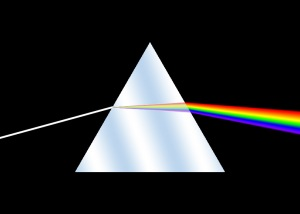
\includegraphics[width=2in]{L5-Prism.jpg}
	\end{figure}


		\item Extension: Integer factorization using quantum computing 	
		
	\end{itemize}

}

\frame{
	\frametitle{DFT: time-domain vs. frequency-domain} 
	\begin{itemize}
		\item DFT, denoted as $\mathbf{X} = \mathcal{F}\{\mathbf{x}\}$,  transforms a sequence of $N$ complex numbers $x_{0}, x_{1}, ..., x_{N-1}$ (time-domain) into 
a $N$-periodic sequence of complex numbers $X_{0}, X_{1}, ..., X_{N-1}$ (frequency-domain): 
\begin{small}
\[
X_{k} = \sum_{n=0}^{N-1} x_{n} e^{ -\frac{2\pi}{N} i kn }, \ \  k=0, 1, ..., N-1
\]
\end{small}
		\item  Here, $X_{k}$ encodes both amplitude and phase of a sinusoidal component $e^{-\frac{2\pi}{N}kn i}$ of the function $x_{n}$ (the sinusoid's frequency is \textcolor{red}{\bf $k$ cycles per $N$ samples}). 
		\item \textcolor{red}{\bf Inverse transform} of DFT: 
\begin{small}
\[
x_{n} = \frac{1}{N}\sum_{k=0}^{N-1} X_{k} e^{ \frac{2\pi}{N}i kn}
\]		    
\end{small}
		An interpretation of DFT is that its inverse transform  is the \textcolor{red}{\bf discrete analogy} of the formula  for  \textcolor{red}{\bf   a Fourier series}:
\begin{small}
\[
f(x)  = \sum_{n=-\infty}^{+\infty} F_{n} e^{ inx}, \ F_{n} = \frac{1}{2\pi} \int_{-\infty}^{\infty} f(x) e^{-inx} \mathrm{d} x
\]		    
\end{small}


%	 	Discrete Fourier transform (DFT) converts a finite sequence of equally-spaced samples of a function into an equivalent-length sequence of equally-spaced samples of the discrete-time Fourier transform (DTFT), which is a complex-valued function of frequency. The interval at which the DTFT is sampled is the reciprocal of the duration of the input sequence. 
%		\item 
%	 The DFT is therefore said to be a frequency domain representation of the original input sequence. 
%	 		\item 
% If the original sequence spans all the non-zero values of a function, its DTFT is continuous (and periodic), and the DFT provides discrete samples of one cycle.
% 		\item 
% If the original sequence is one cycle of a periodic function, the DFT provides all the non-zero values of one DTFT cycle.
% \item The DFT (bottom) computes discrete samples of the continuous DTFT. The inverse DFT (top) is a periodic summation of the original samples. The FFT algorithm computes one cycle of the DFT and its inverse is one cycle of the DFT inverse.
	\end{itemize}
}

\frame{
	\frametitle{Time-frequency transformation}
	
	\begin{itemize}
		\item FFT transforms the input data $a_0, a_1, ..., a_{n-1}$ (time-domain samples) into $y_0, y_1, ..., y_{n-1}$ (frequency domain).  For example, 
	\end{itemize}	
\begin{footnotesize}
\[
\begin{array}{lllllllllllllllllllllllllllll}
y_{0} = a_{0}&+\  a_{1}&+\   a_{2} &+\   a_{3}&+\   a_{4}&+\  a_{5}&+\  a_{6}&+\   a_{7} \nonumber  \\
y_{1} = a_{0}&+\   a_{1}\omega^{1} &+\   a_{2}\omega^{2} &+\   a_{3}\omega^{3} &+\  a_{4}\omega^{4} &+\  a_{5}\omega^{5} &+\   a_{6}\omega^{6} &+\  a_{7}\omega^{7}  \nonumber \\  
y_{2} = a_{0}&+\   a_{1}\omega^{2} &+\   a_{2}\omega^{4} &+\   a_{3}\omega^{6} &+\  a_{4}\omega^{8} &+\  a_{5}\omega^{10} &+\   a_{6}\omega^{12} &+\  a_{7}\omega^{14}  \nonumber \\  
y_{3} = a_{0}&+\   a_{1}\omega^{3} &+\   a_{2}\omega^{6} &+\   a_{3}\omega^{9} &+\  a_{4}\omega^{12} &+\  a_{5}\omega^{15} &+\   a_{6}\omega^{18} &+\  a_{7}\omega^{21}  \nonumber \\  
y_{4} = a_{0}&+\  a_{1}\omega^{4} &+\   a_{2} &+\   a_{3}\omega^{12} &+\  
a_{4}\omega^{16} &+\  a_{5}\omega^{20} &+\  a_{6}\omega^{24} &+\  
a_{7}\omega^{28}  \nonumber \\  
y_{5} = a_{0}&+\   a_{1}\omega^{5} &+\   a_{2}\omega^{10} &+\   a_{3}\omega^{15} &+\  a_{4}\omega^{20} &+\  a_{5}\omega^{25} &+\   a_{6}\omega^{30} &+\  a_{7}\omega^{35}  \nonumber \\  
y_{6} = a_{0}&+\   a_{1}\omega^{6} &+\   a_{2}\omega^{12} &+\   a_{3}\omega^{18} &+\  a_{4}\omega^{24} &+\  a_{5}\omega^{30} &+\   a_{6}\omega^{36} &+\  a_{7}\omega^{42}  \nonumber \\  
y_{7} = a_{0}&+\   a_{1}\omega^{7} &+\   a_{2}\omega^{14} &+\   a_{3}\omega^{21} &+\  a_{4}\omega^{28} &+\  a_{5}\omega^{35} &+\   a_{6}\omega^{42} &+\  a_{7}\omega^{49}  \nonumber 
\end{array}
\]
\end{footnotesize}
	\begin{itemize}
		\item Here $y_{k}$ encodes both amplitude and phase of a sinusoidal component of the time-domain samples  $a_0, a_1, ..., a_7$. 
	\end{itemize}

}

\frame{
		\frametitle{FFT: an example}

		\begin{tt}
			N = 8; \\
			t = 0:1/N:1-1/N; \\
			a = 1*cos(2*pi*1*t) + 2*sin(2*pi*3*t); \\
			Freq = 0:N-1; \\
			bar( Freq, abs(fft(a)), "b", 0.2 );
		\end{tt}
	\begin{figure}
		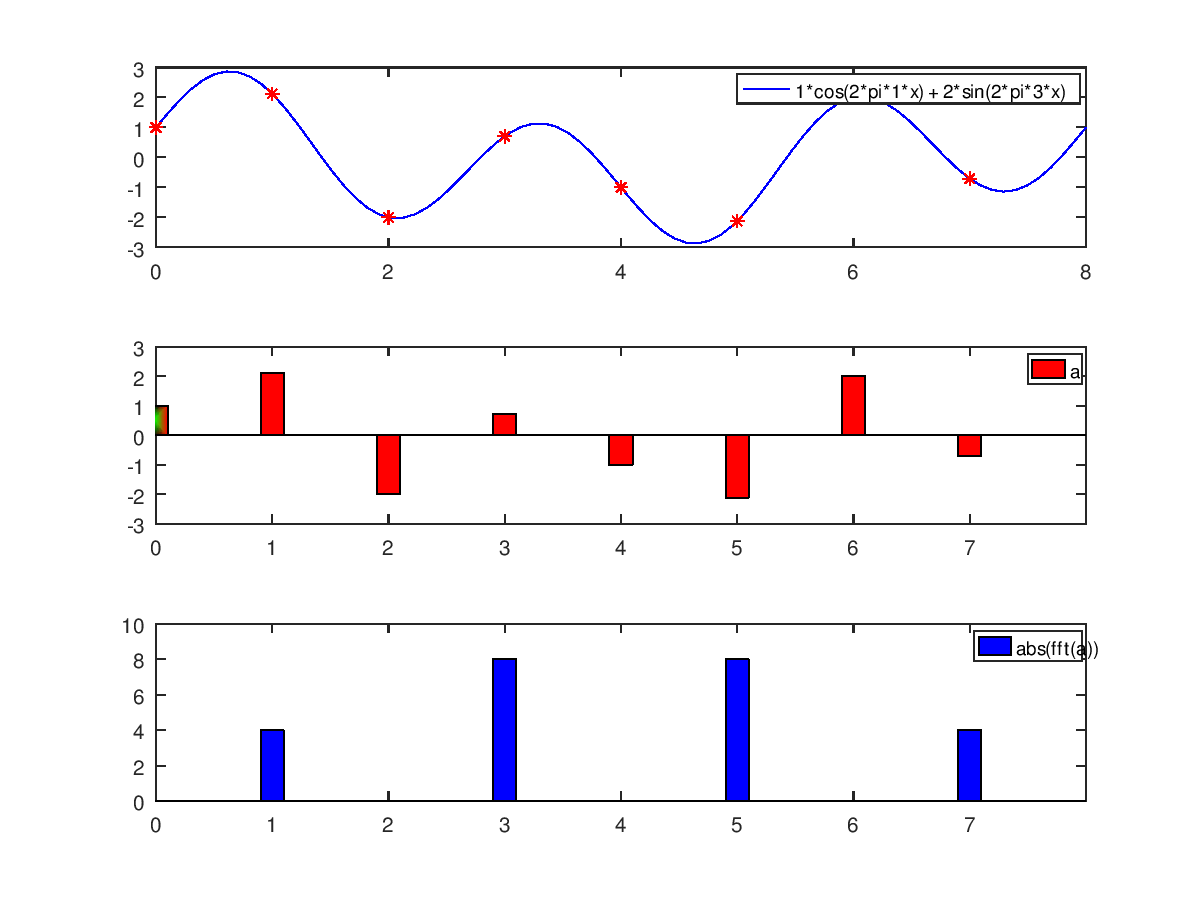
\includegraphics[width=3in]{L5-FFT-demo-x-a-ffta.png} 
	\end{figure}
} 

\frame{
	\frametitle{$y_k$ encodes amplitude and phase of a sinusoidal component}

	\begin{itemize}
		\begin{small}
		\item $y_{k} = a_{0} + a_{1}\omega^{k}  +   a_{2}\omega^{2k}  +  \hdots  +  a_{7}\omega^{7k}$ computes the dot product of two vectors: the time-domain samples $a_0, a_1, ..., a_7$, and a sinusoid signal $1, \omega^{k}, \omega^{2k}, ..., \omega^{7k}$. Here $\omega=e^{\tfrac{2\pi}{8}i}$ and thus the sinusoid has frequency of $k$ cycles per $8$ samples.
		\item The dot product $y_{k}  = 0$ if the time-domain samples $a_0, a_1, ..., a_7$ do not consist of any sinusoidal component of such frequency. The reason is that: 
			\begin{itemize}
				\item The dot product of these two vectors $y_{k} = \sum_{j = 0}^7 a_j \omega^{jk}$ is essentially a discrete analogy of the integral of two sinusoids, say  $\int_{0}^{2\pi}  \cos mx \cdot \cos nx  \mathrm{d} x.$    
				\item The orthogonality of sinusoids states that for two integers $m, n$, 
	\begin{small}
	$$\int_{0}^{2\pi} \cos mx \cdot \sin nx \mathrm{d} x = 0, \text{and}$$ 
	$$\int_{0}^{2\pi} \sin mx \cdot \sin nx \mathrm{d} x = 0, \int_{0}^{2\pi} \cos mx \cdot \cos nx \mathrm{d} x = 0 \ (m\neq n)$$ 
	\end{small}
			\end{itemize}
%			\begin{footnotesize}	
%				\begin{tt}
%a = [1 2.1 -2 0.7 -1 -2.1 2 -0.7] \\
%c = [1 0.7 0 -0.7 -1 -0.7 0 0.7 ]\\
%s = [0 0.7 1 0.7 0 -0.7 -1 -0.7 ]\\
%  sqrt( (a*c')$\wedge$2 + (a*s')$\wedge$2 ) = 4
%  				\end{tt}
%			\end{footnotesize}
		\end{small}
%		\begin{figure}
%			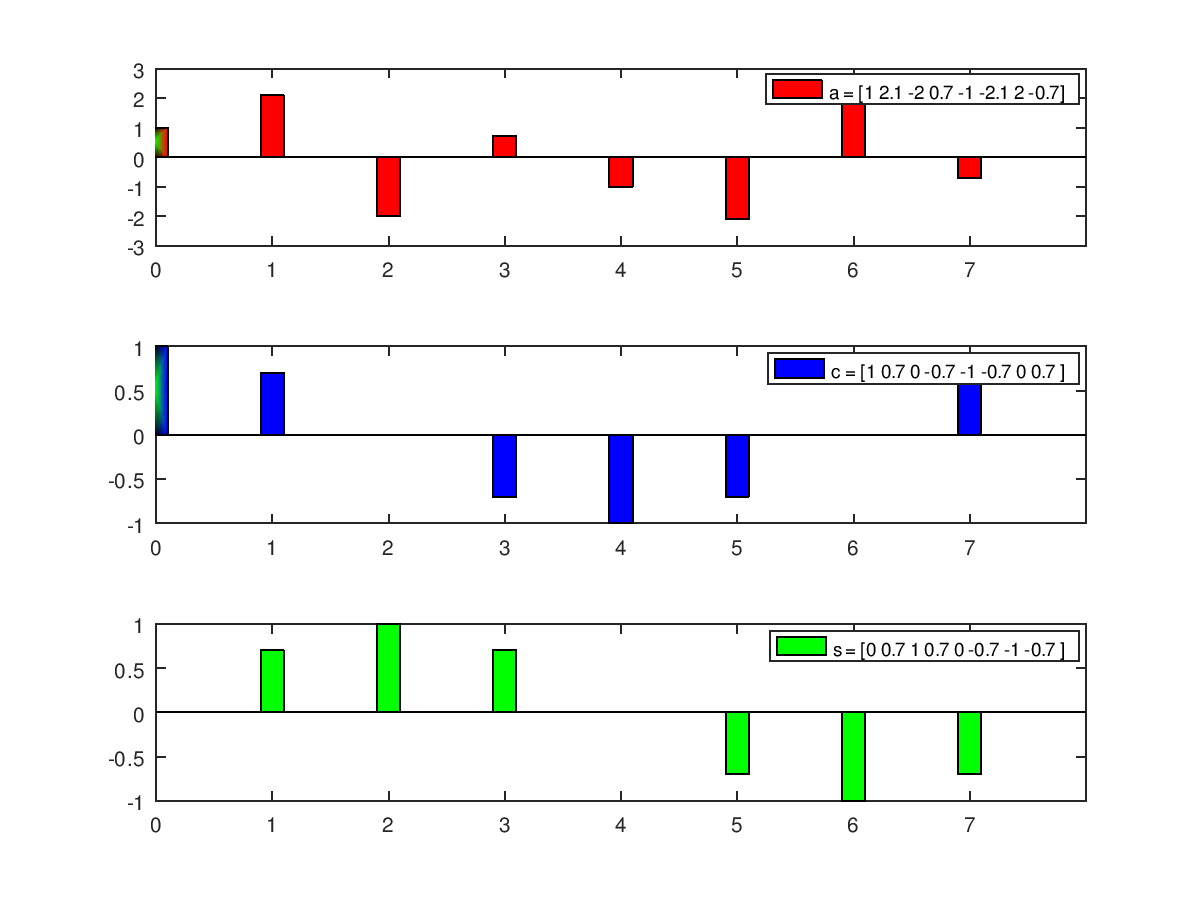
\includegraphics[width=3.0in]{L5-FFT-demo-x-a-ffta-k1.png}
%		\end{figure}

	\end{itemize}
}

\frame{
	\frametitle{Calculation of $y_1$ } 

	\begin{itemize}
		\begin{small}
		\item  $1, \omega^{1}, \omega^{2}, ..., \omega^{7}$ represents a sinusoidal signal of frequency $1$ cycle per $8$ samples, and the existence of such sinusoidal component in the time-domain samples   $a_0, a_1, ..., a_7$ is encoded by the dot product $y_{1} = a_{0} +\   a_{1}\omega^{1}  + \   a_{2}\omega^{2}  +  \hdots  +\  a_{7}\omega^{7}$. %Here $\omega=e^{\tfrac{2\pi}{8}  i}$.
		\item 	\begin{footnotesize}	
				\begin{tt}
a = [1 2.1 -2 0.7 -1 -2.1 2 -0.7] \\
c = [1 0.7 0 -0.7 -1 -0.7 0 0.7 ]\\
s = [0 0.7 1 0.7 0 -0.7 -1 -0.7 ]\\
  sqrt( (a*c')$\wedge$2 + (a*s')$\wedge$2 ) = 4
  				\end{tt}
			\end{footnotesize}
		\end{small}
		\begin{figure}
			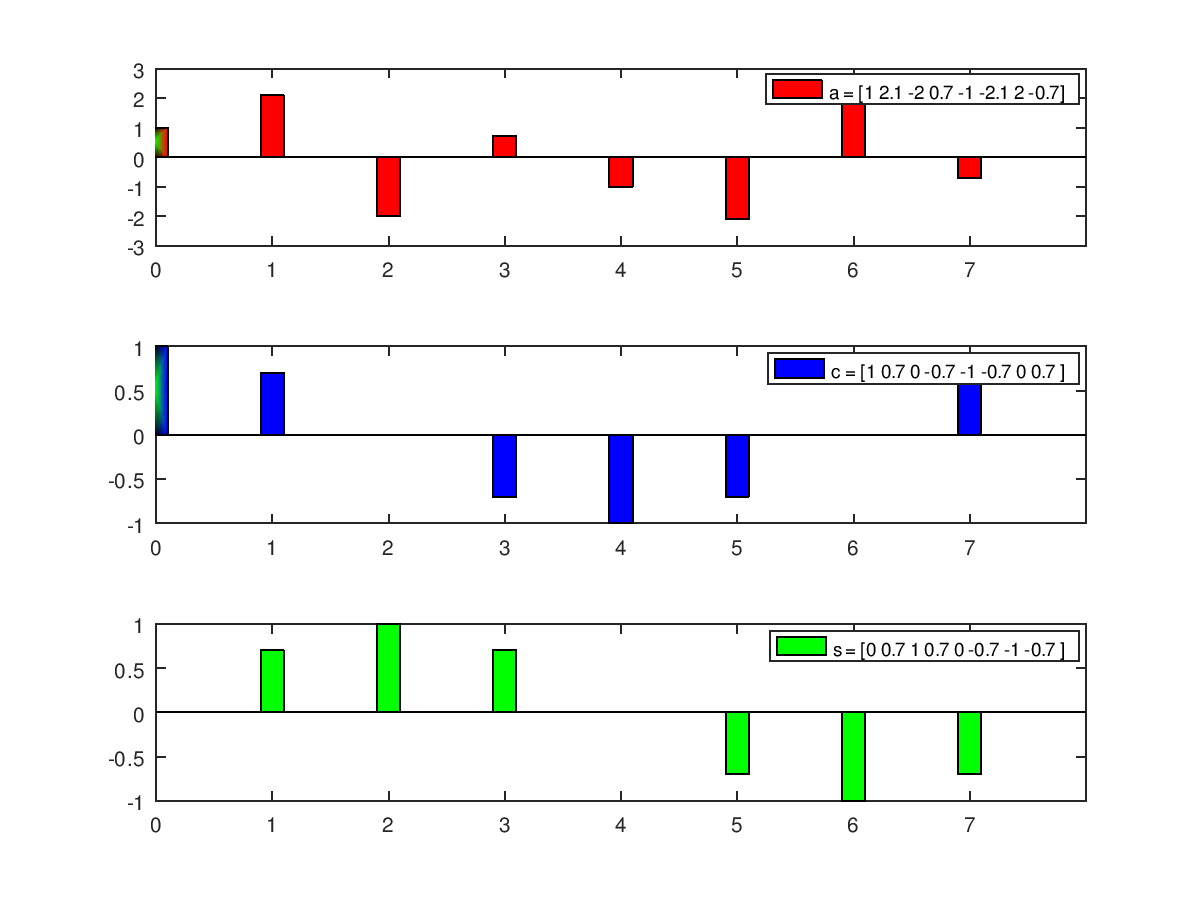
\includegraphics[width=2.8in]{L5-FFT-demo-x-a-ffta-k1.png}
		\end{figure}
	\end{itemize}
}



\frame{
	\frametitle{Calculation of $y_2$}

	
	\begin{itemize}
		\item $1, \omega^{2}, \omega^{4}, ..., \omega^{14}$ represents a sinusoidal signal of frequency $2$ cycles per $8$ samples, and the existence of such sinusoidal component  in   time-domain samples   $a_0, a_1, ..., a_7$ is encoded by the dot product $y_{2} = a_{0} +\   a_{1}\omega^{2}  + \   a_{2}\omega^{4}  +  \hdots  +\  a_{7}\omega^{14}$. %Here $\omega=e^{\tfrac{2\pi}{8}  i}$.
		\item \begin{footnotesize}	
		\begin{tt}
a = [1 2.1 -2 0.7 -1 -2.1 2 -0.7] \\
c = [ 1 0 -1 0 1 0 -1 0 ] \\
s = [ 0 1 0 -1 0 1 0 -1 ] \\
 sqrt( (a*c')$\wedge$2 + (a*s')$\wedge$2 ) = 0
	\begin{figure}
		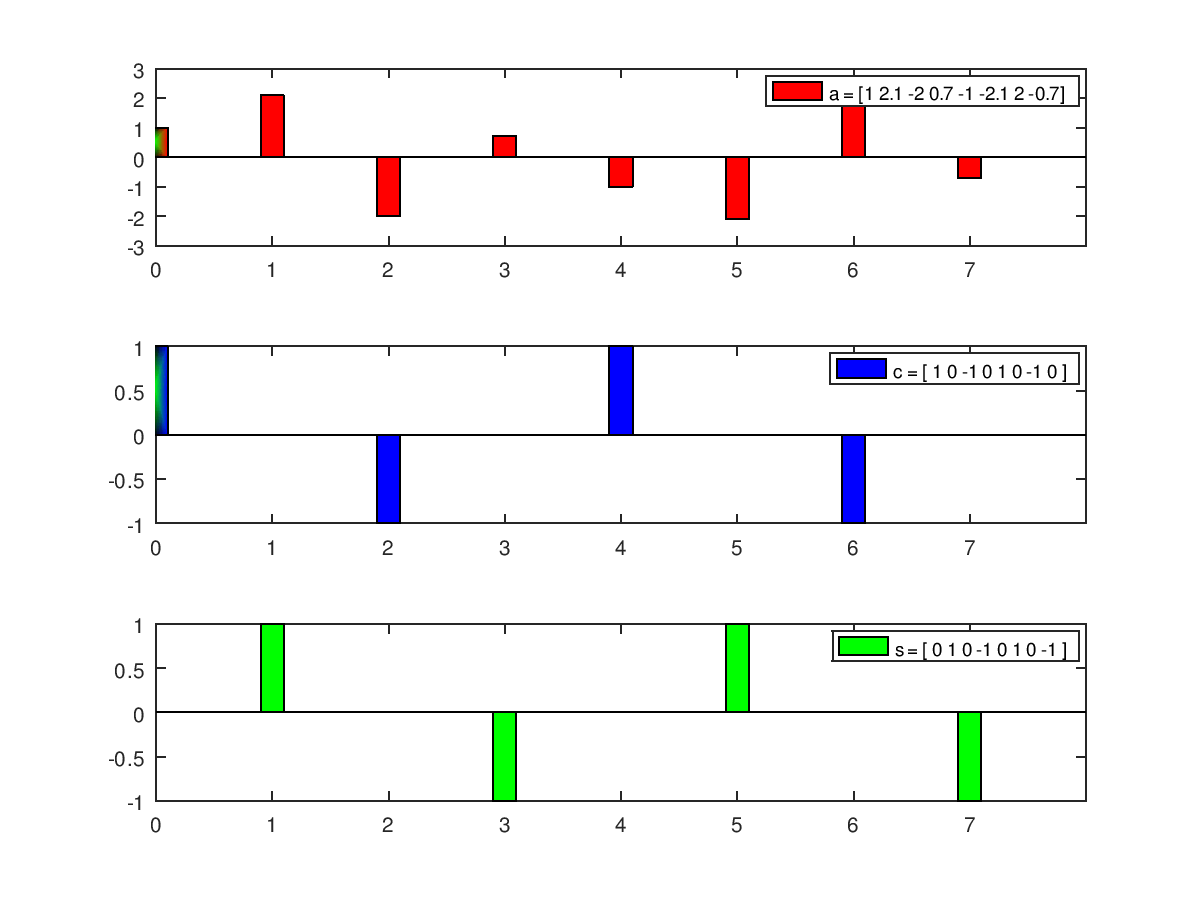
\includegraphics[width=2.8in]{L5-FFT-demo-x-a-ffta-k2.png}
	\end{figure}
		\end{tt}
		\end{footnotesize}
	\end{itemize}
}


\frame{
	\frametitle{Calculation of $y_3$}

	
	\begin{itemize}
		\item $1, \omega^{3}, \omega^{6}, ..., \omega^{21}$ represents a sinusoidal signal of frequency $3$ cycles per $8$ samples, and the existence of such sinusoidal component  in   time-domain samples   $a_0, a_1, ..., a_7$ is encoded by the dot product $y_{3} = a_{0} +\   a_{1}\omega^{3}  + \   a_{2}\omega^{6}  +  \hdots  +\  a_{7}\omega^{21}$. %Here $\omega=e^{\tfrac{2\pi}{8}  i}$.	
		\item \begin{footnotesize}	
		\begin{tt}
a = [1 2.1 -2 0.7 -1 -2.1 2 -0.7]  \\
c = [1 -0.7 0 0.7 -1 0.7 0 -0.7] \\
s = [0 0.7 -1 0.7 0 -0.7 1 -0.7]\\
  sqrt( (a*c')$\wedge$2 + (a*s')$\wedge$2 ) = 8
	\begin{figure}
		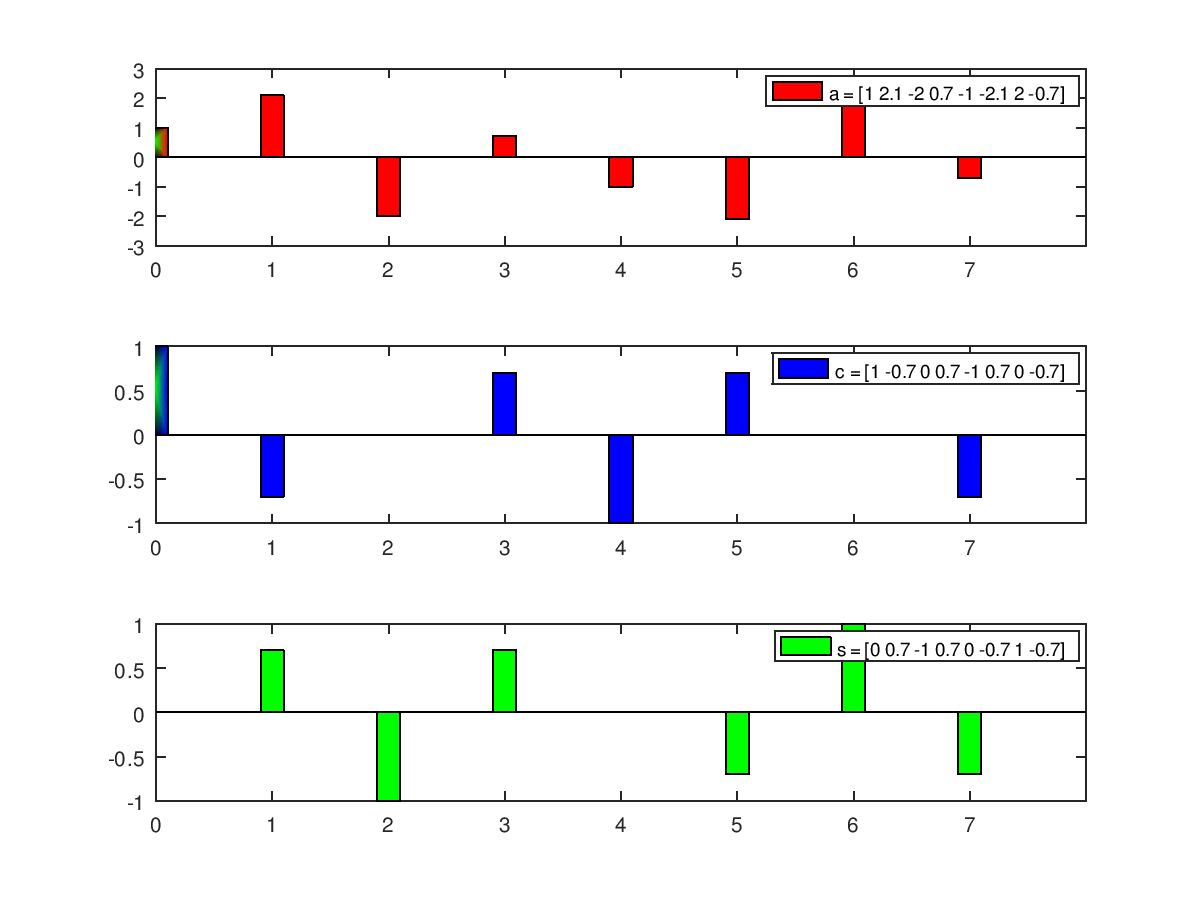
\includegraphics[width=2.8in]{L5-FFT-demo-x-a-ffta-k3.png}
	\end{figure}
		\end{tt}
		\end{footnotesize}
	\end{itemize}
}


\frame{
	\begin{block}{}
	Appendix: Relationship between continuous and discrete Fourier transforms
	 \end{block}

}

\frame{
	\frametitle{Fourier series, Fourier transform, DTFT, and DFT} 
%	\begin{figure}
%		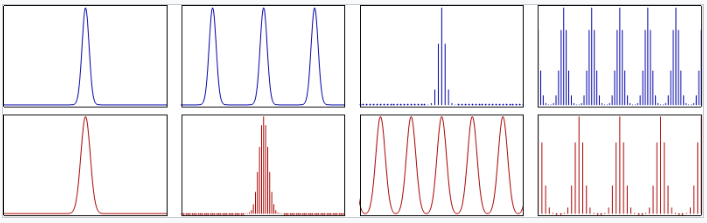
\includegraphics[width=4.5in]{L5-FFT-DTFT.png}; 
%	\end{figure}

	
	\begin{itemize}
		\item Fourier series decomposes a periodic function into a set of sine/cosine waves, and one of the motivations of Fourier transform  comes from the extension of Fourier series to non-periodic functions. 
		\item DTFT uses discrete-time samples of a continuous function as input, and generates a continuous function of frequency. 
		\item Using a finite sequence of equally-spaced samples of a function as input, DFT computes a sequence of identical length, representing equally-spaced samples of DTFT.  The interval at which the DTFT is sampled is reciprocal of the duration of the input sequence. 	
		\item The inverse DFT is a Fourier series using the DTFT samples as coefficients of corresponding frequency, and it is essentially a periodic summation of the original input sequence. 
	\end{itemize}
}

\frame{
	\frametitle{Fourier series: history}
	\begin{figure}
		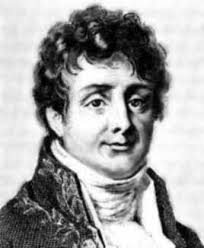
\includegraphics[width=0.8in]{Fourier.jpg}
		\caption{Jean-Baptiste Joseph Fourier (1768-1830)}
	\end{figure}

	\begin{itemize}
		\item  In 1807, Joseph Fourier proposed the idea of Fourier series when solving heat equation, a  partial differential equation. 
		\item Prior to Fourier's work, no solution to  heat equation was known in the general case. However, when the heat source was a simple sine or cosine wave, solutions were known (called eigensolutions). 
		\item Thus, Fourier modelled complicated heat source as a superposition of simple sine/cosine waves, and rewrote the solution as superposition of corresponding eigensolutions. 
%		$$  \frac{1}{\pi} \int_{0}^{2\pi} f(x) \cos nx dx$$
	\end{itemize}
 }


\frame{
	\frametitle{Fourier series}
	
	\begin{itemize}
		\item Fourier series is a way to represent a \textcolor{red}{\bf periodic function} of time as the sum of a set of simple sines and cosines (or, equivalently, complex exponentials).   For example,  the Fourier series of a periodic function $f(x)$ (period  $2\pi$) is:   
\begin{small}		
\[
		 f(x) = a_{0} + \sum_{n=1}^{\infty} (a_{n} \cos nx + b_{n} \sin nx )
\]
\end{small}
where
\begin{small}
$$ a_{0} = \frac{1}{2 \pi} \int_{0}^{2\pi} f(t) \mathrm{d} t$$   
		$$ a_{n} = \frac{1}{\pi} \int_{0}^{2\pi} f(t) \cos nt  \mathrm{d} t \quad (n=1, 2, ...) $$   
		$$ b_{n} = \frac{1}{\pi} \int_{0}^{2\pi} f(t) \sin nt  \mathrm{d} t \quad (n=1, 2, ...) $$ 
\end{small}

\end{itemize}

} 

\frame{
	\frametitle{Fourier series: orthogonality of basis functions}
	
	\begin{itemize}
		\item Unlike Taylor's expansion, the basis functions of Fourier series are orthogonal over $[0, 2\pi]$, i.e., for two integers $m, n$, 
\begin{small}
$$  \int_{0}^{2\pi} 1\cdot \sin x  \mathrm{d} x = 0,\quad  \int_{0}^{2\pi} 1\cdot \cos x  \mathrm{d} x = 0$$   
 $$  \int_{0}^{2\pi}  \sin mx \cdot  \sin nx  \mathrm{d} x = 0,\quad  \int_{0}^{2\pi} \cos mx \cdot \cos nx \mathrm{d} x = 0 \quad (m \neq n)$$    
 $$  \int_{0}^{2\pi}  \cos mx \cdot \sin nx  \mathrm{d} x = 0$$    
\end{small}
		\item The orthogonality plays an important role in solving coefficients $a_0, a_n, b_n$. 
  
\end{itemize}
} 


\frame{
	\frametitle{Fourier series: complex exponential form}
	
	\begin{itemize}
		\item According to the Euler's formula $e^{ix} = \cos x + i \sin x$, we have 
			$ \cos x = \frac{1}{2}(e^{ix} + e^{-ix})$, 
			$ \sin x = \frac{1}{2i}(e^{ix} - e^{-ix})$, and 
		\begin{small}
			\begin{eqnarray}
				 f(x) &=& a_{0} + \sum_{n=1}^{\infty} (a_{n} \cos nx + b_{n} \sin nx ) \nonumber \\ 
				 &=& a_{0} +  \sum_{n=1}^{\infty} ( a_{n} \frac{1}{2}(e^{inx} + e^{-inx}) +  b_{n} \frac{1}{2i}(e^{inx} - e^{-inx} ) )   \nonumber\\
				 &=&  a_{0} +  \sum_{n=1}^{\infty} ( \frac{1}{2} (a_{n} - i b_{n}) e^{inx}
+  \frac{1}{2} (a_{n} + i b_{n}) e^{-inx}  )		\nonumber
	\end{eqnarray}
\end{small}
		\item Define $F_0 = a_{0}$, and $F_{n} = \frac{1}{2} (a_{n} - i b_{n})$ $(n>0)$. We have $F_{-n} = \frac{1}{2} (a_{n} + i b_{n})$, and thus rewrite the Fourier series as: 
\begin{small}		
	$$f(x)  = \sum_{n=-\infty}^{+\infty} F_{n} e^{inx}, F_{n} = \frac{1}{2} (a_{n} - i b_{n}) = \frac{1}{2\pi}  \int_{0}^{2\pi} f(t) e^{-int} \mathrm{d} t$$
\end{small}
	\item Complex exponential form is necessary as the complex coefficients $F_{n}$ (called {\it frequency spectrum}) could encode both amplitude and phase of basic waves. 	 
\end{itemize}

} 

 
 \frame{
 	\frametitle{Fourier series: example 1}
	
	\begin{itemize}
		\item Periodic function $f(x) = \begin{cases}  \frac{1}{2} (\pi - x) & 0<x \leq2\pi \\ 
		f(x+2\pi) & \text{otherwise}
		\end{cases} $

\begin{figure}

	 \begin{tikzpicture}

% horizontal axis
\draw[->] (-3.5,0) -- (3.5,0) node[anchor=north] {\tiny $x$};
% labels
\draw	(0,0) node[anchor=north west] {\tiny $0$}
		(1,0) node[anchor=north] {\tiny $\pi$}
		(2,0) node[anchor=north] {\tiny $2\pi$}
		(3,0) node[anchor=north] {\tiny $3\pi$}
		(-1,0) node[anchor=north] {\tiny $-\pi$}
		(-2,0) node[anchor=north] {\tiny $-2\pi$}
		(-3,0) node[anchor=north] {\tiny $-3\pi$};

%draw ticks on X
\def\d{0.04};
\draw [thick] (1, 0+\d) -- (1, 0); 
\draw [thick] (2, 0+\d) -- (2, 0); 
\draw [thick] (3, 0+\d) -- (3, 0); 
\draw [thick] (-1, 0+\d) -- (-1, 0); 
\draw [thick] (-2, 0+\d) -- (-2, 0); 
\draw [thick] (-3, 0+\d) -- (-3, 0); 

% vertical axis
\draw[->] (0,-1) -- (0,1) node[anchor=east] {\tiny  $f(x)$};
%draw ticks on Y
\def\d{0.04};
\draw [thick] ( 0+\d, 0.5) -- ( 0, 0.5); 
\draw [thick] (0+\d, -0.5) -- (0, -0.5); 
%draw Label on Y
\draw	(0, 0.5) node[anchor=east] {\tiny $\frac{\pi}{2}$};
\draw	(0, -0.5) node[anchor=east] {\tiny $-\frac{\pi}{2}$};





% f(x)
\draw[thick] (0,0.5) -- (2,-0.5);
\draw[thick] (0,-0.5) -- (-2,0.5);
\draw[thick] (3, 0) -- (2,0.5);
\draw[thick] (-3, 0) -- (-2,-0.5);


%circles 
\draw[fill=white, draw] (0, 0.5) circle (1pt);
\draw[fill=white, draw] (-2, 0.5) circle (1pt);
\draw[fill=white, draw] (2, 0.5) circle (1pt);


\end{tikzpicture}
\end{figure}
		\item Fourier series: $f(x) =  \sum_{n=1}^{\infty} \frac{1}{n} \sin nx$ (since $a_{n} = 0$, $b_{n} = \frac{1}{n}$)
		
\begin{figure}

	 \begin{tikzpicture}

% horizontal axis
\draw[->] (-3.5,0) -- (3.5,0) node[anchor=north] {\tiny $x$};
% labels
\draw	(0,0) node[anchor=north west] {\tiny $0$}
		(1,0) node[anchor=north] {\tiny $\pi$}
		(2,0) node[anchor=north] {\tiny $2\pi$}
		(3,0) node[anchor=north] {\tiny $3\pi$}
		(-1,0) node[anchor=north] {\tiny $-\pi$}
		(-2,0) node[anchor=north] {\tiny $-2\pi$}
		(-3,0) node[anchor=north] {\tiny $-3\pi$};

%draw ticks on X
\def\d{0.04};
\draw [thick] (1, 0+\d) -- (1, 0); 
\draw [thick] (2, 0+\d) -- (2, 0); 
\draw [thick] (3, 0+\d) -- (3, 0); 
\draw [thick] (-1, 0+\d) -- (-1, 0); 
\draw [thick] (-2, 0+\d) -- (-2, 0); 
\draw [thick] (-3, 0+\d) -- (-3, 0); 

% vertical axis
\draw[->] (0,-1) -- (0,1) node[anchor=east] {\tiny  $f(x)$};
%draw ticks on Y
\def\d{0.04};
\draw [thick] ( 0+\d, 0.5) -- ( 0, 0.5); 
\draw [thick] (0+\d, -0.5) -- (0, -0.5); 
%draw Label on Y
\draw	(0, 0.5) node[anchor=east] {\tiny $\frac{\pi}{2}$};
\draw	(0, -0.5) node[anchor=east] {\tiny $-\frac{\pi}{2}$};



%
%
%% f(x)
%\draw[thick] (0,0.5) -- (2,-0.5);
%\draw[thick] (0,-0.5) -- (-2,0.5);
%\draw[thick] (3, 0) -- (2,0.5);
%\draw[thick] (-3, 0) -- (-2,-0.5);
%
%
%%circles 
%\draw[fill=white, draw] (0, 0.5) circle (1pt);
%\draw[fill=white, draw] (-2, 0.5) circle (1pt);
%\draw[fill=white, draw] (2, 0.5) circle (1pt);
%\draw[scale=1,domain=-3:3,smooth,variable=\x,blue] plot ({\x},{sin(\x)});
\draw [green,smooth, samples=100, domain=-3:3] plot (\x, {1/3.1415926*sin(3.1415926*\x r)});
\draw [blue,smooth, samples=100, domain=-3:3] plot (\x, {1/3.1415926* (sin(3.1415926*\x r) + 0.5*sin(2*3.1415926*\x r)     )});
\draw [red,smooth, samples=200, domain=-3:3] plot (\x, {1/3.1415926* (sin(3.1415926*\x r) + 0.5*sin(2*3.1415926*\x r) + 0.33333*sin(3*3.1415926*\x r) + 0.25*sin(4*3.1415926*\x r) + 0.2*sin(5*3.1415926*\x r) + 0.16666666*sin(6*3.1415926*\x r) + 1/7.0*sin(7*3.1415926*\x r) + 1/8.0*sin(8*3.1415926*\x r) + 1/9.0*sin(9*3.1415926*\x r) + 1/10.0*sin(10*3.1415926*\x r) + 1/11.0*sin(11*3.1415926*\x r)  + 1/12.0*sin(12*3.1415926*\x r)  + 1/13.0*sin(13*3.1415926*\x r)  + 1/14.0*sin(14*3.1415926*\x r)   + 1/15.0*sin(15*3.1415926*\x r) + 1/16.0*sin(16*3.1415926*\x r) + 1/17.0*sin(17*3.1415926*\x r)  + 1/18.0*sin(18*3.1415926*\x r)  + 1/19.0*sin(19*3.1415926*\x r) + 1/20.0*sin(20*3.1415926*\x r)        )});

\end{tikzpicture}
\end{figure}
		
	\end{itemize}

 }


\frame{
	\frametitle{Fourier series: extension to $f(x)$ with period of $2L$} 
	
	\begin{itemize}
		\item For a periodic function $f(x)$ with period of $2L$, the Fourier series is: 
				$$  f(x) = a_0 + \sum_{n=1}^\infty (a_n \cos \frac{\pi}{L}nx + b_n \sin \frac{\pi}{L}nx) $$
		\item The coefficients are: 
				$$ a_0 = \frac{1}{2L} \int_0^{2L} f(t) \mathrm{d} t$$	
				$$ a_n = \frac{1}{L} \int_0^{2L} f(t) \cos \frac{\pi}{L} nt \mathrm{d} t$$ 		
				$$ b_n = \frac{1}{L} \int_0^{2L} f(t) \sin \frac{\pi}{L} nt \mathrm{d} t$$ 		
	\end{itemize}
}
	
 
 \frame{
 	\frametitle{Fourier series: example 2}
	
	\begin{itemize}
		\item Periodic function $f(x) = \begin{cases} 1 &  | x | \leq \frac{1}{4}  \\ 
		0 &  \frac{1}{4}  < | x | \leq \frac{T}{2} 
		\end{cases} $, and $f(x)$ has a period $T=1$. 

  \begin{figure}

	 \begin{tikzpicture}

% Draw X Y plane 
\def\startx{-3};
\def\endx{3};
\def\starty{0};
\def\endy{1};
\def\R{0.3};
\def\d{0.04};
\def\DX{0};
\def\DY{0};

%X axis
\draw[->] (\startx - \R + \DX,  0+\DY) -- (\endx + \R + \DX, 0+\DY) node[anchor=north] {\tiny $x$};
% X labels, and ticks
\foreach \i in {\startx,..., \endx}
{
	\ifthenelse{\i = 0} {
		\draw (\i + \DX, 0+\DY ) node[anchor=north west] {\tiny $\i$};
	}{
		\draw (\i + \DX, 0+\DY ) node[anchor=north] {\tiny $\i$};
		\draw [thick] (\i+ \DX,  0+\d+\DY) -- (\i+ \DX,  0+\DY); 
	};
}

% Y axis
\draw[->] (0 + \DX, \starty - \R +\DY) -- (0 + \DX, \endy + \R +\DY) node[anchor=east] {\tiny  $f(x)$};
% Y labels, and ticks 
\foreach \i in {\starty,..., \endy}
{
	\ifthenelse{\i = 0} {;} {
		\draw (0 + \DX, \i+\DY ) node[anchor=east] {\tiny $\i$};
		\draw [thick] (0+ \DX + \d,  \i+\DY) -- (0+ \DX,  \i+\DY); 
	}
}

% f(x)
\def\T{1}; 
\def\t{0.25};
\foreach \n in {-2, -1, 0, 1, 2} {
	\draw[thick, blue] (\n*\T -\t + \DX, 1 + \DY) -- (\n*\T +\t + \DX, 1 + \DY);

	\draw[thick, blue] (\n*\T  -\t + \DX, 0 + \DY) -- (\n*\T -\t + \DX, 1 + \DY);
	\draw[thick, blue] (\n*\T  + \t + \DX, 0 + \DY) -- (\n*\T +\t + \DX, 1 + \DY);

	\draw[thick, blue] (\n*\T + \t + \DX, 0 + \DY) -- (\n*\T +\T-\t + \DX, 0 + \DY);
	\draw[thick, blue] (\n*\T -\t + \DX, 0 + \DY) -- (\n*\T -\T+\t + \DX, 0 + \DY);
} 

\end{tikzpicture}
\end{figure}

		\item Fourier series: $$f(x) = \frac{1}{2T} +  \frac{2}{\pi} \sum_{n=1}^{\infty} \frac{1}{n} \sin (\frac{\pi}{2T}n) \cos(\frac{2\pi}{T}nx)$$
		
\begin{figure}

	 \begin{tikzpicture}

% Draw X Y plane 
\def\startx{-3};
\def\endx{3};
\def\starty{0};
\def\endy{1};
\def\R{0.3};
\def\d{0.04};
\def\DX{0};
\def\DY{0};

%X axis
\draw[->] (\startx - \R + \DX,  0+\DY) -- (\endx + \R + \DX, 0+\DY) node[anchor=north] {\tiny $x$};
% X labels, and ticks
\foreach \i in {\startx,..., \endx}
{
	\ifthenelse{\i = 0} {
		\draw (\i + \DX, 0+\DY ) node[anchor=north west] {\tiny $\i$};
	}{
		\draw (\i + \DX, 0+\DY ) node[anchor=north] {\tiny $\i$};
		\draw [thick] (\i+ \DX,  0+\d+\DY) -- (\i+ \DX,  0+\DY); 
	};
}

% Y axis
\draw[->] (0 + \DX, \starty - \R +\DY) -- (0 + \DX, \endy + \R +\DY) node[anchor=east] {\tiny  $f(x)$};
% Y labels, and ticks 
\foreach \i in {\starty,..., \endy}
{
	\ifthenelse{\i = 0} {;} {
		\draw (0 + \DX, \i+\DY ) node[anchor=east] {\tiny $\i$};
		\draw [thick] (0+ \DX + \d,  \i+\DY) -- (0+ \DX,  \i+\DY); 
	}
}

\def\T{1};
\draw [green,smooth, samples=100, domain=-16:16] plot (\T*\x/2.0/3.1415926, {1.0/\T/2 + 2.0/3.1415926* ( 1.0 / 1.0 *sin(1*3.1415926/\T/2 r) * cos(1*\x  r)                ) } );
\draw [blue,smooth, samples=100, domain=-16:16] plot (\T*\x/2.0/3.1415926, {1.0/\T/2 + 2.0/3.1415926* ( 1.0 / 1.0 *sin(1*3.1415926/\T/2 r) * cos(1*\x  r)  + 1.0 / 2.0 *sin(2*3.1415926/\T/2 r) * cos(2*\x  r)  + 1.0 / 3.0 *sin(3*3.1415926/\T/2 r) * cos(3*\x  r)  + 1.0 / 4.0 *sin(4*3.1415926/\T/2 r) * cos(4*\x  r)              ) } );
\draw [red,smooth, samples=100, domain=-16:16] plot (\T*\x/2.0/3.1415926, {1.0/\T/2 + 2.0/3.1415926* ( 1.0 / 1.0 *sin(1*3.1415926/\T/2 r) * cos(1*\x  r)  + 1.0 / 2.0 *sin(2*3.1415926/\T/2 r) * cos(2*\x  r)  + 1.0 / 3.0 *sin(3*3.1415926/\T/2 r) * cos(3*\x  r)  + 1.0 / 4.0 *sin(4*3.1415926/\T/2 r) * cos(4*\x  r)  + 1.0 / 5.0 *sin(5*3.1415926/\T/2 r) * cos(5*\x  r)  + 1.0 / 6.0 *sin(6*3.1415926/\T/2 r) * cos(6*\x  r) + 1.0 /7.0 *sin(7*3.1415926/\T/2 r) * cos(7*\x  r)  + 1.0 / 8.0 *sin(8*3.1415926/\T/2 r) * cos(8*\x  r)           ) } );

\end{tikzpicture}
\end{figure}
		
	\end{itemize}

 }

 \frame{
 	\frametitle{Convergence of Fourier series: Dirichlet's conditions}

	\begin{itemize}
		\item Dirichlet's theorem states the sufficient conditions for the convergence of Fourier series, i.e.,  if $f(x)$ satisfies the following conditions:    	
		\begin{enumerate}
			\item $f(x)$ is periodic, and  absolutely integrable over a period; 
			\item $f(x)$ must have a  finite number of maxima and minima in any bounded interval; 
			\item $f(x)$ must have a finite number of discontinuities in any bounded interval, and the discontinuity cannot be infinite. 
		\end{enumerate}
		Then  $$a_{0} + \sum_{n=1}^{m}(a_{n} \cos nx + b_{n} \sin nx) \rightarrow \frac{1}{2}( f(x+0) + f(x-0) ) $$	when $m\rightarrow \infty$. 
		\item A succinct proof using Dirac's $\delta$ function can be found in {\it Mathematical Methods for Physics} (by Q. Gu). 
	\end{itemize}
 }

\frame{
\begin{proof}
	 \begin{itemize}
	 	\item Since \begin{small} 
		$a_{n} \cos nx + b_{n} \sin nx = \frac{1}{\pi} {\displaystyle \int_{-\pi}^{\pi}} f(t) \cos n(x-t) \mathrm{d} t$\end{small}, the partial sum of Fourier series is: 
	 \begin{small}	
	 	\begin{eqnarray}
			S_{m}(x) &=& \frac{1}{2\pi} \int_{-\pi}^{\pi}   f(t) [ 1 + 2\sum_{n=1}^{m} \cos n (x-t) ]   \mathrm{d} t \nonumber  \\  
	 			&=& \int_{-\pi}^{\pi}  f(t) \frac{ \sin ( (m+\frac{1}{2}) (x-t) )}{ 2\pi \sin\frac{1}{2}(x-t) } \mathrm{d} t \nonumber\\ 
				&=& \int_{-\pi}^{\pi}  f(t) D_{m}(x-t) \mathrm{d} t   \nonumber
		\end{eqnarray}
		
		\item Here $D_{m}(x) = \frac{1}{2\pi}( 1 + 2\cos x + 2\cos 2x + ... + 2 \cos mx )$. 
		\item Note that $\lim_{m\rightarrow \infty} D_{m}(x) = \delta(x)$ since  \begin{small} ${\displaystyle \int_{-\pi}^{\pi}} D_{m}(x) \mathrm{d} x = 1$\end{small} and \begin{small} $D_{m}(0) = \frac{1}{2\pi} (2m+1)\rightarrow \infty$\end{small}. 
		\item Thus, we have  \begin{small}$ {\displaystyle \lim_{m\rightarrow \infty}} S_{m}	 (x) =  {\displaystyle \int_{-\pi}^{\pi}}  f(t)  \delta(x-t) = f(x)$  \end{small} (when $f(x)$ is continous at $x$). 
		 Please refer to  {\it Mathematical Methods for Physics} (by Q. Gu) for complete proof. 
	 \end{small}
	 \end{itemize}
 \end{proof}

} 
 
 \frame{
 	\frametitle{Fourier transform (in terms of angular frequency $\omega$)}
	 \begin{itemize}
	 	\item Fourier transform of a function of time (a {\it signal}) is a complex-valued function of frequency (represented as  {\it angular frequency} $\omega$), whose absolute value represents the amount of that frequency present in the original function. 
		\begin{footnotesize}
		$$ F(\omega) = \int_{-\infty}^{\infty} f(x) e^{-i x \omega} \mathrm{d} x, \ f(x) = \frac{1}{2\pi} \int_{-\infty}^{\infty} F(\omega) e^{i\omega x} \mathrm{d} \omega$$
		\end{footnotesize}
		\item Fourier transform, denoted as $F(\omega) = \mathcal{F}\{f(x)\}$, is called {\it frequency representation of the original signal}, and $F(\omega)$ is called {\it  spectral density}. 
		\item For example,  the Fourier transform of \begin{footnotesize} 
 $f(x) = \begin{cases}
								1 & | x | \leq \frac{1}{4} \\ 
								0 & \text{otherwise}
							\end{cases}$  \end{footnotesize}
				is \begin{footnotesize}  $$F(\omega) = \int_{-\infty}^\infty f(x) e^{-i\omega x} \mathrm{d} x = \frac{2}{\omega} \sin (\frac{\omega}{4})$$  	\end{footnotesize}						
		\end{itemize}
		
 \begin{figure}

	 \begin{tikzpicture}

% Draw X Y plane 
\def\startx{-2};
\def\endx{2};
\def\starty{0};
\def\endy{1};
\def\R{0.3};
\def\d{0.04};
\def\DX{0};
\def\DY{0};

%X axis
\draw[->] (\startx - \R + \DX,  0+\DY) -- (\endx + \R + \DX, 0+\DY) node[anchor=north] {\tiny $x$};
% X labels, and ticks
\foreach \i in {\startx,..., \endx}
{
	\ifthenelse{\i = 0} {
		\draw (\i + \DX, 0+\DY ) node[anchor=north west] {\tiny $\i$};
	}{
		\draw (\i + \DX, 0+\DY ) node[anchor=north] {\tiny $\i$};
		\draw [thick] (\i+ \DX,  0+\d+\DY) -- (\i+ \DX,  0+\DY); 
	};
}

% Y axis
\draw[->] (0 + \DX, \starty - \R +\DY) -- (0 + \DX, \endy + \R +\DY) node[anchor=east] {\tiny  $f(x)$};
% Y labels, and ticks 
\foreach \i in {\starty,..., \endy}
{
	\ifthenelse{\i = 0} {;} {
		\draw (0 + \DX, \i+\DY ) node[anchor=east] {\tiny $\i$};
		\draw [thick] (0+ \DX + \d,  \i+\DY) -- (0+ \DX,  \i+\DY); 
	}
}

% f(x)
\def\T{1}; 
\def\t{0.25};
\foreach \n in { 0 } {
	\draw[thick, blue] (\n*\T -\t + \DX, 1 + \DY) -- (\n*\T +\t + \DX, 1 + \DY);

	\draw[thick, blue] (\n*\T  -\t + \DX, 0 + \DY) -- (\n*\T -\t + \DX, 1 + \DY);
	\draw[thick, blue] (\n*\T  + \t + \DX, 0 + \DY) -- (\n*\T +\t + \DX, 1 + \DY);

	\draw[thick, blue] (\n*\T + \t + \DX, 0 + \DY) -- (\n*\T +\T-\t + \DX, 0 + \DY);
	\draw[thick, blue] (\n*\T -\t + \DX, 0 + \DY) -- (\n*\T -\T+\t + \DX, 0 + \DY);
} 
	\draw[thick, blue] (0*\T + \t + \DX, 0 + \DY) -- (0*\T +\T-\t + 0.7 + \DX, 0 + \DY);
	\draw[thick, blue] (0*\T -\t + \DX, 0 + \DY) -- (0*\T -\T+\t  - 0.7 + \DX, 0 + \DY);


%% horizontal axis
%\draw[->] (-2.7,0) -- (2.7,0) node[anchor=north] {\tiny $x$};
%% labels
%\draw	(0,0) node[anchor=north west] {\tiny $0$};
%\draw		(1,0) node[anchor=north] {\tiny $1$};
%\draw		(-1,0) node[anchor=north] {\tiny $-1$};
%\draw		(2,0) node[anchor=north] {\tiny $2$};
%\draw		(-2,0) node[anchor=north] {\tiny $-2$};
%
%%draw ticks on X
%\def\d{0.04};
%\draw [thick] (1, 0+\d) -- (1, 0); 
%\draw [thick] (-1, 0+\d) -- (-1, 0); 
%\draw [thick] (2, 0+\d) -- (2, 0); 
%\draw [thick] (-2, 0+\d) -- (-2, 0); 
%
%% Y axis
%\draw[->] (0,-0.3) -- (0,1.3) node[anchor=east] {\tiny  $f(x)$};
%%draw ticks on Y
%\def\d{0.04};
%\draw [thick] ( 0+\d, 1) -- ( 0, 1); 
%%\draw [thick] (0+\d, -1) -- (0, -1); 
%%draw Label on Y
%\draw	(0, 1) node[anchor=east] {\tiny $1$};
%%\draw	(0, -1) node[anchor=east] {\tiny $-1$};
%
%% f(x)
%\def\T{1.5}; 
%\draw[thick, blue] (-0.5, 0) -- (-0.5, 1);
%\draw[thick, blue] (-0.5, 1) -- (0.5, 1);
%\draw[thick, blue] (0.5, 0) -- (0.5, 1);
%\draw[thick, blue] (0.5, 0) -- (2.5, 0);
%
%\draw[thick, blue] (-0.5, 0) -- (-2.5, 0);
%



\def\DX{6};
\def\DY{0};


%F(w) 
% x axis
\draw[->] (-2.3+\DX, 0+\DY) -- (2.3++\DX, 0+\DY) node[anchor=north] {\tiny $\omega$};
 labels
\draw	(0+\DX,0+\DY) node[anchor=north west] {\tiny $0$};
\draw		(1+\DX,0+\DY) node[anchor=north] {\tiny $4\pi$};
\draw		(-1+\DX,0+\DY) node[anchor=north] {\tiny $-4\pi$};
\draw		(2+\DX,0+\DY) node[anchor=north] {\tiny $8\pi$};
\draw		(-2+\DX,0+\DY) node[anchor=north] {\tiny $-8\pi$};

%draw ticks on X
\def\d{0.04};
\draw [thick] (1+\DX, 0+\d+\DY) -- (1+\DX, 0+\DY); 
\draw [thick] (-1+\DX, 0+\d+\DY) -- (-1+\DX, 0+\DY); 
\draw [thick] (2+\DX, 0+\d+\DY) -- (2+\DX, 0+\DY); 
\draw [thick] (-2+\DX, 0+\d+\DY) -- (-2+\DX, 0+\DY); 

% Y axis
\draw[->] (0+\DX,-0.3+\DY) -- (0+\DX,1.3+\DY) node[anchor=east] {\tiny  $F(\omega)$};
%draw ticks on Y
\def\d{0.04};
\draw [thick] ( 0+\d+\DX, 1+\DY) -- ( 0+\DX, 1+\DY); 
%\draw [thick] (0+\d, -1) -- (0, -1); 
%draw Label on Y
\draw	(0+\DX, 1+\DY) node[anchor=east] {\tiny $1$};
%\draw	(0, -1) node[anchor=east] {\tiny $-1$};

%plot F(w) 

\draw [red,smooth, samples=100, domain=-30:30] plot (\x/3.1415926/4 + \DX, { sin(\x/4 r)*2/\x       +\DY} );

\end{tikzpicture}
\end{figure}
 }


 \frame{
 	\frametitle{Fourier transform (in terms of ordinary frequency $\nu$) }
	 \begin{itemize}
	 	\item For a sinusoidal wave with period $T$ (measured in {\it seconds}), its frequency can be measured using angular frequency $\omega$ (measured in {\it radians per second}) or using ordinary frequency $\nu$ (measured in {\it cycles per second}, or hertz), where $\omega = 2\pi \nu$, and $\nu = \frac{1}{T}$. 
		\item  When using angular frequency $\omega$,  Fourier transform is defined as: 
		\begin{footnotesize}
		$$ F(\omega) = \int_{-\infty}^{\infty} f(x) e^{-i x \omega} \mathrm{d} x$$
		$$ f(x) = \frac{1}{2\pi} \int_{-\infty}^{\infty} F(\omega) e^{i\omega x} \mathrm{d} \omega$$ 		
		\end{footnotesize}
		\item  Replacing $\omega$ with $\omega = 2\pi \nu$, we obtain another representation of  Fourier transform in terms of ordinary frequency $\nu$: 
		\begin{footnotesize}
		$$ F(\nu) = \int_{-\infty}^{\infty} f(x) e^{- 2\pi i x \nu} \mathrm{d} x$$
		$$ f(x) =  \int_{-\infty}^{\infty} F(\nu) e^{2\pi i  x \nu} \mathrm{d} \nu $$
		\end{footnotesize}

		\end{itemize}
}
 

 \frame{
 	\frametitle{Connection between Fourier series and Fourier transform}
	 \begin{itemize}
		\item \begin{small}
For a function that are zero outside an interval, we can calculate Fourier series on any larger interval. As we lengthen the interval, the coefficients of Fourier series will approach Fourier transform. 	\end{small}

	 \end{itemize}
	 
	 

\begin{figure}
	 \begin{tikzpicture}

% T = 1
% Draw X Y plane 
\def\startx{-2};
\def\endx{2};
\def\starty{0};
\def\endy{1};
\def\R{0.3};
\def\d{0.04};
\def\DX{0};
\def\DY{4};

%X axis
\draw[->] (\startx - \R + \DX,  0+\DY) -- (\endx + \R + \DX, 0+\DY) node[anchor=north] {\tiny $x$};
% X labels, and ticks
\foreach \i in {\startx,..., \endx}
{
	\ifthenelse{\i = 0} {
		\draw (\i + \DX, 0+\DY ) node[anchor=north west] {\tiny $\i$};
	}{
		\draw (\i + \DX, 0+\DY ) node[anchor=north] {\tiny $\i$};
		\draw [thick] (\i+ \DX,  0+\d+\DY) -- (\i+ \DX,  0+\DY); 
	};
}

% Y axis
\draw[->] (0 + \DX, \starty - \R +\DY) -- (0 + \DX, \endy + \R +\DY) node[anchor=east] {\tiny  $f(x)$};
\draw[->] (0 + \DX, \starty - \R +\DY) -- (0 + \DX, \endy + \R +\DY) node[anchor=west, blue, thick] {\tiny  $T=1$};
% Y labels, and ticks 
\foreach \i in {\starty,..., \endy}
{
	\ifthenelse{\i = 0} {;} {
		\draw (0 + \DX, \i+\DY ) node[anchor=east] {\tiny $\i$};
		\draw [thick] (0+ \DX + \d,  \i+\DY) -- (0+ \DX,  \i+\DY); 
	}
}

% f(x)
% f(x)
\def\T{1}; 
\def\t{0.25};
\foreach \n in {-2, -1, 0, 1, 2} {
	\draw[thick, blue] (\n*\T -\t + \DX, 1 + \DY) -- (\n*\T +\t + \DX, 1 + \DY);

	\draw[thick, blue] (\n*\T  -\t + \DX, 0 + \DY) -- (\n*\T -\t + \DX, 1 + \DY);
	\draw[thick, blue] (\n*\T  + \t + \DX, 0 + \DY) -- (\n*\T +\t + \DX, 1 + \DY);

	\draw[thick, blue] (\n*\T + \t + \DX, 0 + \DY) -- (\n*\T +\T-\t + \DX, 0 + \DY);
	\draw[thick, blue] (\n*\T -\t + \DX, 0 + \DY) -- (\n*\T -\T+\t + \DX, 0 + \DY);
} 



\def\DX{6};
\def\DY{4};

%F(w) 
% x axis
\draw[->] (-2.3+\DX, 0+\DY) -- (2.3++\DX, 0+\DY) node[anchor=north] {\tiny $\omega$};
 labels
\draw	(0+\DX,0+\DY) node[anchor=north west] {\tiny $0$};
\draw		(1+\DX,0+\DY) node[anchor=north] {\tiny $4\pi$};
\draw		(-1+\DX,0+\DY) node[anchor=north] {\tiny $-4\pi$};
\draw		(2+\DX,0+\DY) node[anchor=north] {\tiny $8\pi$};
\draw		(-2+\DX,0+\DY) node[anchor=north] {\tiny $-8\pi$};

%draw ticks on X
\def\d{0.04};
\draw [thick] (1+\DX, 0+\d+\DY) -- (1+\DX, 0+\DY); 
\draw [thick] (-1+\DX, 0+\d+\DY) -- (-1+\DX, 0+\DY); 
\draw [thick] (2+\DX, 0+\d+\DY) -- (2+\DX, 0+\DY); 
\draw [thick] (-2+\DX, 0+\d+\DY) -- (-2+\DX, 0+\DY); 

% Y axis
\draw[->] (0+\DX,-0.3+\DY) -- (0+\DX,1.3+\DY) node[anchor=east] {\tiny  $2\pi\frac{F_{n}}{\omega}$};
%draw ticks on Y
\def\d{0.04};
\draw [thick] ( 0+\d+\DX, 1+\DY) -- ( 0+\DX, 1+\DY); 
%\draw [thick] (0+\d, -1) -- (0, -1); 
%draw Label on Y
\draw	(0+\DX, 1+\DY) node[anchor=east] {\tiny $1$};
%\draw	(0, -1) node[anchor=east] {\tiny $-1$};

%plot F(w) 

\draw [dashed, red,smooth, samples=100, domain=-30:30] plot (\x/3.1415926/4 + \DX, { sin(\x/4 r)*2/\x       +\DY} );
\def\w{2*3.1415926/\T};
\foreach \i in {-3,...,3}
{
	\ifthenelse{\i = 0}{
		\draw[blue, thick] ( 0 + \DX, 0 +\DY) -- (0 + \DX,  { 1/2  +\DY} ); 
	}{
		\draw[blue, thick] ( \i*2*3.1415926/\T/3.1415926/4 + \DX, 0 +\DY) -- (\i*2*3.1415926/\T/3.1415926/4 + \DX,  { sin(\i*2*3.1415926/\T/4 r)*2/(\i*2*3.1415926/\T)     +\DY} ); 
	}	
}
\node[ blue, thick, above] at (1 + \DX, 0.5 +\DY) {\tiny $\Delta\omega = 2\pi$}; 






% Draw X Y plane 
\def\startx{-2};
\def\endx{2};
\def\starty{0};
\def\endy{1};
\def\R{0.3};
\def\d{0.04};
\def\DX{0};
\def\DY{2};

%X axis
\draw[->] (\startx - \R + \DX,  0+\DY) -- (\endx + \R + \DX, 0+\DY) node[anchor=north] {\tiny $x$};
% X labels, and ticks
\foreach \i in {\startx,..., \endx}
{
	\ifthenelse{\i = 0} {
		\draw (\i + \DX, 0+\DY ) node[anchor=north west] {\tiny $\i$};
	}{
		\draw (\i + \DX, 0+\DY ) node[anchor=north] {\tiny $\i$};
		\draw [thick] (\i+ \DX,  0+\d+\DY) -- (\i+ \DX,  0+\DY); 
	};
}

% Y axis
\draw[->] (0 + \DX, \starty - \R +\DY) -- (0 + \DX, \endy + \R +\DY) node[anchor=east] {\tiny  $f(x)$};
\draw[->] (0 + \DX, \starty - \R +\DY) -- (0 + \DX, \endy + \R +\DY) node[anchor=west, blue, thick] {\tiny  $T=2$};
% Y labels, and ticks 
\foreach \i in {\starty,..., \endy}
{
	\ifthenelse{\i = 0} {;} {
		\draw (0 + \DX, \i+\DY ) node[anchor=east] {\tiny $\i$};
		\draw [thick] (0+ \DX + \d,  \i+\DY) -- (0+ \DX,  \i+\DY); 
	}
}

% f(x)
% f(x)
\def\T{2}; 
\def\t{0.25};
\foreach \n in {  0 } {
	\draw[thick, blue] (\n*\T -\t + \DX, 1 + \DY) -- (\n*\T +\t + \DX, 1 + \DY);

	\draw[thick, blue] (\n*\T  -\t + \DX, 0 + \DY) -- (\n*\T -\t + \DX, 1 + \DY);
	\draw[thick, blue] (\n*\T  + \t + \DX, 0 + \DY) -- (\n*\T +\t + \DX, 1 + \DY);

	\draw[thick, blue] (\n*\T + \t + \DX, 0 + \DY) -- (\n*\T +\T-\t + \DX, 0 + \DY);
	\draw[thick, blue] (\n*\T -\t + \DX, 0 + \DY) -- (\n*\T -\T+\t + \DX, 0 + \DY);
} 

\foreach \n in {  1 } {
	\draw[thick, blue] (\n*\T -\t + \DX, 1 + \DY) -- (\n*\T +\t + \DX, 1 + \DY);

	\draw[thick, blue] (\n*\T  -\t + \DX, 0 + \DY) -- (\n*\T -\t + \DX, 1 + \DY);
	\draw[thick, blue] (\n*\T  + \t + \DX, 0 + \DY) -- (\n*\T +\t + \DX, 1 + \DY);

	\draw[thick, blue] (\n*\T + \t + \DX, 0 + \DY) -- (\n*\T +\t +0.2 + \DX, 0 + \DY);
	\draw[thick, blue] (\n*\T -\t + \DX, 0 + \DY) -- (\n*\T -\T+\t + \DX, 0 + \DY);
} 

\foreach \n in {  -1 } {
	\draw[thick, blue] (\n*\T -\t + \DX, 1 + \DY) -- (\n*\T +\t + \DX, 1 + \DY);

	\draw[thick, blue] (\n*\T  -\t + \DX, 0 + \DY) -- (\n*\T -\t + \DX, 1 + \DY);
	\draw[thick, blue] (\n*\T  + \t + \DX, 0 + \DY) -- (\n*\T +\t + \DX, 1 + \DY);

	\draw[thick, blue] (\n*\T + \t + \DX, 0 + \DY) -- (\n*\T +\T-\t + \DX, 0 + \DY);
	\draw[thick, blue] (\n*\T -\t + \DX, 0 + \DY) -- (\n*\T -\t-0.3 + \DX, 0 + \DY);
} 



\def\DX{6};
\def\DY{2};

%F(w) 
% x axis
\draw[->] (-2.3+\DX, 0+\DY) -- (2.3++\DX, 0+\DY) node[anchor=north] {\tiny $\omega$};
 labels
\draw	(0+\DX,0+\DY) node[anchor=north west] {\tiny $0$};
\draw		(1+\DX,0+\DY) node[anchor=north] {\tiny $4\pi$};
\draw		(-1+\DX,0+\DY) node[anchor=north] {\tiny $-4\pi$};
\draw		(2+\DX,0+\DY) node[anchor=north] {\tiny $8\pi$};
\draw		(-2+\DX,0+\DY) node[anchor=north] {\tiny $-8\pi$};

%draw ticks on X
\def\d{0.04};
\draw [thick] (1+\DX, 0+\d+\DY) -- (1+\DX, 0+\DY); 
\draw [thick] (-1+\DX, 0+\d+\DY) -- (-1+\DX, 0+\DY); 
\draw [thick] (2+\DX, 0+\d+\DY) -- (2+\DX, 0+\DY); 
\draw [thick] (-2+\DX, 0+\d+\DY) -- (-2+\DX, 0+\DY); 

% Y axis
\draw[->] (0+\DX,-0.3+\DY) -- (0+\DX,1.3+\DY) node[anchor=east] {\tiny  $2\pi\frac{F_{n}}{\omega}$};
%draw ticks on Y
\def\d{0.04};
\draw [thick] ( 0+\d+\DX, 1+\DY) -- ( 0+\DX, 1+\DY); 
%\draw [thick] (0+\d, -1) -- (0, -1); 
%draw Label on Y
\draw	(0+\DX, 1+\DY) node[anchor=east] {\tiny $1$};
%\draw	(0, -1) node[anchor=east] {\tiny $-1$};

%plot F(w) 

\draw [dashed, red,smooth, samples=100, domain=-30:30] plot (\x/3.1415926/4 + \DX, { sin(\x/4 r)*2/\x       +\DY} );
\def\w{2*3.1415926/\T};
\foreach \i in {-8,...,8}
{
	\ifthenelse{\i = 0}{
		\draw[blue, thick] ( 0 + \DX, 0 +\DY) -- (0 + \DX,  { 1/2  +\DY} ); 
	}{
		\draw[blue, thick] ( \i*2*3.1415926/\T/3.1415926/4 + \DX, 0 +\DY) -- (\i*2*3.1415926/\T/3.1415926/4 + \DX,  { sin(\i*2*3.1415926/\T/4 r)*2/(\i*2*3.1415926/\T)     +\DY} ); 
	}	
}

\node[ blue, thick, above] at (1 + \DX, 0.5 +\DY) {\tiny $\Delta\omega = \pi$}; 






% Draw X Y plane 
\def\startx{-2};
\def\endx{2};
\def\starty{0};
\def\endy{1};
\def\R{0.3};
\def\d{0.04};
\def\DX{0};
\def\DY{0};

%X axis
\draw[->] (\startx - \R + \DX,  0+\DY) -- (\endx + \R + \DX, 0+\DY) node[anchor=north] {\tiny $x$};
% X labels, and ticks
\foreach \i in {\startx,..., \endx}
{
	\ifthenelse{\i = 0} {
		\draw (\i + \DX, 0+\DY ) node[anchor=north west] {\tiny $\i$};
	}{
		\draw (\i + \DX, 0+\DY ) node[anchor=north] {\tiny $\i$};
		\draw [thick] (\i+ \DX,  0+\d+\DY) -- (\i+ \DX,  0+\DY); 
	};
}

% Y axis
\draw[->] (0 + \DX, \starty - \R +\DY) -- (0 + \DX, \endy + \R +\DY) node[anchor=east] {\tiny  $f(x)$};
\draw[->] (0 + \DX, \starty - \R +\DY) -- (0 + \DX, \endy + \R +\DY) node[anchor=west, blue, thick] {\tiny  $T=\infty$};
% Y labels, and ticks 
\foreach \i in {\starty,..., \endy}
{
	\ifthenelse{\i = 0} {;} {
		\draw (0 + \DX, \i+\DY ) node[anchor=east] {\tiny $\i$};
		\draw [thick] (0+ \DX + \d,  \i+\DY) -- (0+ \DX,  \i+\DY); 
	}
}

% f(x)
\def\T{1}; 
\def\t{0.25};
\foreach \n in { 0 } {
	\draw[thick, blue] (\n*\T -\t + \DX, 1 + \DY) -- (\n*\T +\t + \DX, 1 + \DY);

	\draw[thick, blue] (\n*\T  -\t + \DX, 0 + \DY) -- (\n*\T -\t + \DX, 1 + \DY);
	\draw[thick, blue] (\n*\T  + \t + \DX, 0 + \DY) -- (\n*\T +\t + \DX, 1 + \DY);

	\draw[thick, blue] (\n*\T + \t + \DX, 0 + \DY) -- (\n*\T +\T-\t + \DX, 0 + \DY);
	\draw[thick, blue] (\n*\T -\t + \DX, 0 + \DY) -- (\n*\T -\T+\t + \DX, 0 + \DY);
} 
	\draw[thick, blue] (0*\T + \t + \DX, 0 + \DY) -- (0*\T +\T-\t + 0.7 + \DX, 0 + \DY);
	\draw[thick, blue] (0*\T -\t + \DX, 0 + \DY) -- (0*\T -\T+\t  - 0.7 + \DX, 0 + \DY);

\def\DX{6};
\def\DY{0};

%F(w) 
% x axis
\draw[->] (-2.3+\DX, 0+\DY) -- (2.3++\DX, 0+\DY) node[anchor=north] {\tiny $\omega$};
 labels
\draw	(0+\DX,0+\DY) node[anchor=north west] {\tiny $0$};
\draw		(1+\DX,0+\DY) node[anchor=north] {\tiny $4\pi$};
\draw		(-1+\DX,0+\DY) node[anchor=north] {\tiny $-4\pi$};
\draw		(2+\DX,0+\DY) node[anchor=north] {\tiny $8\pi$};
\draw		(-2+\DX,0+\DY) node[anchor=north] {\tiny $-8\pi$};

%draw ticks on X
\def\d{0.04};
\draw [thick] (1+\DX, 0+\d+\DY) -- (1+\DX, 0+\DY); 
\draw [thick] (-1+\DX, 0+\d+\DY) -- (-1+\DX, 0+\DY); 
\draw [thick] (2+\DX, 0+\d+\DY) -- (2+\DX, 0+\DY); 
\draw [thick] (-2+\DX, 0+\d+\DY) -- (-2+\DX, 0+\DY); 

% Y axis
\draw[->] (0+\DX,-0.3+\DY) -- (0+\DX,1.3+\DY) node[anchor=east] {\tiny  $F(\omega)$};
%draw ticks on Y
\def\d{0.04};
\draw [thick] ( 0+\d+\DX, 1+\DY) -- ( 0+\DX, 1+\DY); 
%\draw [thick] (0+\d, -1) -- (0, -1); 
%draw Label on Y
\draw	(0+\DX, 1+\DY) node[anchor=east] {\tiny $1$};
%\draw	(0, -1) node[anchor=east] {\tiny $-1$};

%plot F(w) 

\draw [red,smooth, samples=100, domain=-30:30] plot (\x/3.1415926/4 + \DX, { sin(\x/4 r)*2/\x       +\DY} );
\end{tikzpicture}
\end{figure}
 }
 
 
 
  \frame{
 	\frametitle{Fourier transform: deduction}
	 \begin{itemize}
	 	\item Consider a periodic function $f(x)$ with period $2L$.  Its Fourier series $f(x) = a_0 + \sum_{n=1}^\infty (a_n \cos \frac{\pi}{L}n x + b_n  \sin \frac{\pi}{L} nx)$ can be rewritten as $f(x) = a_0 + \sum_{n=1}^\infty (a_n \cos \omega_n x + b_n  \sin \omega_n x)$, where $\omega_n = \frac{\pi}{L} n$ represents angular frequency.  
		\item Intuitively, when $L\rightarrow \infty$, $f(x)$ becomes a non-periodic function over $(-\infty, \infty)$, and \begin{footnotesize} $$ \sum_{n=1}^\infty ... \Delta \omega \rightarrow \int_0^\infty ... \mathrm{d} \omega.$$ \end{footnotesize}   
		\item In particular, we have $a_0 = \frac{1}{2L} \int_{-L}^L f(t) \mathrm{d} t \xrightarrow{L\rightarrow\infty} 0$ since $f(x)$ is absolutely integrable, and 
\begin{footnotesize}
		\begin{eqnarray}
			\sum_{n=1}^{\infty} a_n \cos \omega_n x &=& \sum_{n=1}^{\infty} \frac{1}{L}  \big[ \int_{-L}^{L} f(t) \cos \omega_n t \mathrm{d} t \big] \cos \omega_n x \nonumber \\ 
			&=& \sum_{n=1}^{\infty} \frac{\Delta \omega}{\pi}  \big[ \int_{-L}^{L} f(t) \cos \omega_n t \mathrm{d} t \big]   \cos \omega_n x \nonumber \\    
			&\rightarrow& \int_0^\infty \mathrm{d} \omega \big[ \frac{1}{\pi} \int_{-\infty}^\infty f(t) \cos \omega t \mathrm{d} t \big] \cos \omega x  \nonumber
		\end{eqnarray}
\end{footnotesize}

	 \end{itemize}
 }

\frame{
 	\frametitle{Fourier transform: deduction cont'd } 
	 \begin{itemize}
		\item Similarly, we have  \begin{footnotesize}
		$$\sum_{n=1}^{\infty} b_n \sin \omega_n x \rightarrow  \int_0^\infty \mathrm{d} \omega \big[ \frac{1}{\pi} \int_{-\infty}^\infty f(t) \sin \omega t \mathrm{d} t \big] \sin \omega x$$\end{footnotesize} and rewrite Fourier series as: 
	\begin{footnotesize}
		\begin{eqnarray}
		f(x) &=& \frac{1}{\pi} \int_{\omega=0}^\infty \int_{t=-\infty}^\infty  f(t) ( \cos \omega x \cos \omega t + \sin \omega x \sin \omega t ) \mathrm{d} t \mathrm{d} \omega 	 \nonumber \\ 
		&=&  \frac{1}{\pi} \int_{\omega=0}^\infty \int_{t=-\infty}^\infty  f(t) \cos \omega (x-t)  \mathrm{d} t \mathrm{d} \omega  \nonumber \\ 
		&=&  \frac{1}{2\pi} \int_{\omega=0}^\infty \int_{t=-\infty}^\infty  f(t) (e^{i\omega (x-t)} + e^{-i\omega (x-t)})  \mathrm{d} t \mathrm{d} \omega  \nonumber \\ 
		&=& \frac{1}{2\pi} \int_{-\infty}^\infty \big[ \int_{0}^\infty f(t)e^{i\omega (x-t)} \mathrm{d} \omega + \int_{0}^\infty f(t) e^{-i\omega (x-t)} \mathrm{d} \omega \big] \mathrm{d} t \nonumber \\  
		&=& \frac{1}{2\pi} \int_{-\infty}^\infty  \int_{-\infty}^\infty f(t)e^{i\omega (x-t)} \mathrm{d} \omega \mathrm{d} t \nonumber \\  
		&=& \frac{1}{2\pi} \int_{-\infty}^\infty F(\omega) \mathrm{d} t \nonumber
		\end{eqnarray}
	\end{footnotesize}		
 	 \end{itemize}
} 

\frame{
 	\frametitle{Fourier transform: properties}
	\begin{itemize}
		\item Linear operations performed in one domain (time or frequency) have corresponding operations in the other domain. 
		\item Differentiation in time domain corresponds to multiplication in the frequency domain, usually making it easier to analyze. 
		\item Convolution in the time domain corresponds to the ordinary multiplication the frequency domain. 
		\item Functions that are localized in one domain have Fourier transforms that are spread out across the other domain, known as the {\it uncertainty principle}. 
		\item The Fourier transform of a Gaussian function is another Gaussian function.
		 
	\end{itemize}


}

\frame{
	\frametitle{Fourier transform: Poisson summation formula}
	
	
	\begin{itemize}
		\item For a function $f(x)$ with its Fourier transform (in terms of ordinary frequency) \begin{footnotesize}$F(\nu) = {\displaystyle \int_{-\infty}^{\infty}} f(x) e^{-2\pi i x \nu} \mathrm{d} x$\end{footnotesize}, the Poisson summation formula states 
		\begin{footnotesize}$ \sum\limits_{k=-\infty}^{\infty} f(k) = \sum\limits_{k=-\infty}^{\infty} F(k) $.\end{footnotesize}
%	\end{itemize}
%}
%	
%\frame{
%	\frametitle{Poisson summation formula: an example}
%
%	\begin{itemize}
	
		\item For example,  the Fourier transform of \begin{footnotesize} 
 $f(x) = \begin{cases}
								1 & | x | \leq \frac{1}{4} \\ 
								0 & \text{otherwise}
							\end{cases}$  \end{footnotesize}
				is \begin{footnotesize}  $$F(\nu) = \int_{-\infty}^\infty f(x) e^{- 2\pi i\nu x} \mathrm{d} x = \frac{1}{\pi \nu } \sin (\frac{\pi \nu}{2})$$  	\end{footnotesize}		
				
		\item Poisson summation formula states that 		
			\begin{center}\begin{footnotesize}$ \sum\limits_{k=-\infty}^{\infty} f(k) = 1 = \sum\limits_{k=-\infty}^{\infty} F(k) $.\end{footnotesize}	\end{center}			
	\end{itemize}
		
 \begin{figure}

	 \begin{tikzpicture}

% Draw X Y plane 
\def\startx{-2};
\def\endx{2};
\def\starty{0};
\def\endy{1};
\def\R{0.3};
\def\d{0.04};
\def\DX{0};
\def\DY{0};

%X axis
\draw[->] (\startx - \R + \DX,  0+\DY) -- (\endx + \R + \DX, 0+\DY) node[anchor=north] {\tiny $x$};
% X labels, and ticks
\foreach \i in {\startx,..., \endx}
{
	\ifthenelse{\i = 0} {
		\draw (\i + \DX, 0+\DY ) node[anchor=north west] {\tiny $\i$};
	}{
		\draw (\i + \DX, 0+\DY ) node[anchor=north] {\tiny $\i$};
		\draw [thick] (\i+ \DX,  0+\d+\DY) -- (\i+ \DX,  0+\DY); 
	};
}

% Y axis
\draw[->] (0 + \DX, \starty - \R +\DY) -- (0 + \DX, \endy + \R +\DY) node[anchor=east] {\tiny  $f(x)$};
% Y labels, and ticks 
\foreach \i in {\starty,..., \endy}
{
	\ifthenelse{\i = 0} {;} {
		\draw (0 + \DX, \i+\DY ) node[anchor=east] {\tiny $\i$};
		\draw [thick] (0+ \DX + \d,  \i+\DY) -- (0+ \DX,  \i+\DY); 
	}
}

% f(x)
\def\T{1}; 
\def\t{0.25};
\foreach \n in { 0 } {
	\draw[thick, blue] (\n*\T -\t + \DX, 1 + \DY) -- (\n*\T +\t + \DX, 1 + \DY);

	\draw[thick, blue] (\n*\T  -\t + \DX, 0 + \DY) -- (\n*\T -\t + \DX, 1 + \DY);
	\draw[thick, blue] (\n*\T  + \t + \DX, 0 + \DY) -- (\n*\T +\t + \DX, 1 + \DY);

	\draw[thick, blue] (\n*\T + \t + \DX, 0 + \DY) -- (\n*\T +\T-\t + \DX, 0 + \DY);
	\draw[thick, blue] (\n*\T -\t + \DX, 0 + \DY) -- (\n*\T -\T+\t + \DX, 0 + \DY);
} 
	\draw[thick, blue] (0*\T + \t + \DX, 0 + \DY) -- (0*\T +\T-\t + 0.7 + \DX, 0 + \DY);
	\draw[thick, blue] (0*\T -\t + \DX, 0 + \DY) -- (0*\T -\T+\t  - 0.7 + \DX, 0 + \DY);


%% horizontal axis
%\draw[->] (-2.7,0) -- (2.7,0) node[anchor=north] {\tiny $x$};
%% labels
%\draw	(0,0) node[anchor=north west] {\tiny $0$};
%\draw		(1,0) node[anchor=north] {\tiny $1$};
%\draw		(-1,0) node[anchor=north] {\tiny $-1$};
%\draw		(2,0) node[anchor=north] {\tiny $2$};
%\draw		(-2,0) node[anchor=north] {\tiny $-2$};
%
%%draw ticks on X
%\def\d{0.04};
%\draw [thick] (1, 0+\d) -- (1, 0); 
%\draw [thick] (-1, 0+\d) -- (-1, 0); 
%\draw [thick] (2, 0+\d) -- (2, 0); 
%\draw [thick] (-2, 0+\d) -- (-2, 0); 
%
%% Y axis
%\draw[->] (0,-0.3) -- (0,1.3) node[anchor=east] {\tiny  $f(x)$};
%%draw ticks on Y
%\def\d{0.04};
%\draw [thick] ( 0+\d, 1) -- ( 0, 1); 
%%\draw [thick] (0+\d, -1) -- (0, -1); 
%%draw Label on Y
%\draw	(0, 1) node[anchor=east] {\tiny $1$};
%%\draw	(0, -1) node[anchor=east] {\tiny $-1$};
%
%% f(x)
%\def\T{1.5}; 
%\draw[thick, blue] (-0.5, 0) -- (-0.5, 1);
%\draw[thick, blue] (-0.5, 1) -- (0.5, 1);
%\draw[thick, blue] (0.5, 0) -- (0.5, 1);
%\draw[thick, blue] (0.5, 0) -- (2.5, 0);
%
%\draw[thick, blue] (-0.5, 0) -- (-2.5, 0);
%



\def\DX{6};
\def\DY{0};


%F(w) 
% x axis
\draw[->] (-2.3+\DX, 0+\DY) -- (2.3++\DX, 0+\DY) node[anchor=north] {\tiny $\omega$};
 labels
\draw	(0+\DX,0+\DY) node[anchor=north west] {\tiny $0$};
\draw		(1+\DX,0+\DY) node[anchor=north] {\tiny $4\pi$};
\draw		(-1+\DX,0+\DY) node[anchor=north] {\tiny $-4\pi$};
\draw		(2+\DX,0+\DY) node[anchor=north] {\tiny $8\pi$};
\draw		(-2+\DX,0+\DY) node[anchor=north] {\tiny $-8\pi$};

%draw ticks on X
\def\d{0.04};
\draw [thick] (1+\DX, 0+\d+\DY) -- (1+\DX, 0+\DY); 
\draw [thick] (-1+\DX, 0+\d+\DY) -- (-1+\DX, 0+\DY); 
\draw [thick] (2+\DX, 0+\d+\DY) -- (2+\DX, 0+\DY); 
\draw [thick] (-2+\DX, 0+\d+\DY) -- (-2+\DX, 0+\DY); 

% Y axis
\draw[->] (0+\DX,-0.3+\DY) -- (0+\DX,1.3+\DY) node[anchor=east] {\tiny  $F(\nu)$};
%draw ticks on Y
\def\d{0.04};
\draw [thick] ( 0+\d+\DX, 1+\DY) -- ( 0+\DX, 1+\DY); 
%\draw [thick] (0+\d, -1) -- (0, -1); 
%draw Label on Y
\draw	(0+\DX, 1+\DY) node[anchor=east] {\tiny $1$};
%\draw	(0, -1) node[anchor=east] {\tiny $-1$};

%plot F(w) 

\draw [red,smooth, samples=100, domain=-30:30] plot (\x/3.1415926/4 + \DX, { sin(3.14159 * \x/2 r)/ ( \x * 3.14159)   +\DY} );

%Poisson
\end{tikzpicture}
\end{figure}

}


\frame{
 	\frametitle{DTFT}
	\begin{itemize}
		\item Discrete-time Fourier transform (DTFT) refers to Fourier analysis on the uniformly-spaced samples of a continuous function, i.e., a Fourier series with $x_{n}$ as coefficients: 
		\begin{footnotesize}
$$ X(\omega) = \sum_{n=-\infty}^{\infty} x_{n} e^{-in\omega}$$ 
		\end{footnotesize}
		Here, the frequency variable $\omega$ has normalized units of $radians/sample$. 
	\end{itemize}
 \begin{figure}
	
	 \begin{tikzpicture}

% Draw X Y plane 
\def\startx{-2};
\def\endx{2};
\def\starty{0};
\def\endy{1};
\def\R{0.3};
\def\d{0.04};
\def\DX{0};
\def\DY{0};

%X axis
\draw[->] (\startx - \R + \DX,  0+\DY) -- (\endx + \R + \DX, 0+\DY) node[anchor=north] {\tiny $x$};
% X labels, and ticks
\foreach \i in {\startx,..., \endx}
{
	\ifthenelse{\i = 0} {
		\draw (\i + \DX, 0+\DY ) node[anchor=north west] {\tiny $\i$};
	}{
		\draw (\i + \DX, 0+\DY ) node[anchor=north] {\tiny $\i$};
		\draw [thick] (\i+ \DX,  0+\d+\DY) -- (\i+ \DX,  0+\DY); 
	};
}

% Y axis
\draw[->] (0 + \DX, \starty - \R +\DY) -- (0 + \DX, \endy + \R +\DY) node[anchor=east] {\tiny  $f(x)$};
% Y labels, and ticks 
\foreach \i in {\starty,..., \endy}
{
	\ifthenelse{\i = 0} {;} {
		\draw (0 + \DX, \i+\DY ) node[anchor=east] {\tiny $\i$};
		\draw [thick] (0+ \DX + \d,  \i+\DY) -- (0+ \DX,  \i+\DY); 
	}
}

% f(x)
\def\T{1}; 
\def\t{0.25};
\foreach \n in { 0 } {
	\draw[thick, blue] (\n*\T -\t + \DX, 1 + \DY) -- (\n*\T +\t + \DX, 1 + \DY);

	\draw[thick, blue] (\n*\T  -\t + \DX, 0 + \DY) -- (\n*\T -\t + \DX, 1 + \DY);
	\draw[thick, blue] (\n*\T  + \t + \DX, 0 + \DY) -- (\n*\T +\t + \DX, 1 + \DY);

	\draw[thick, blue] (\n*\T + \t + \DX, 0 + \DY) -- (\n*\T +\T-\t + \DX, 0 + \DY);
	\draw[thick, blue] (\n*\T -\t + \DX, 0 + \DY) -- (\n*\T -\T+\t + \DX, 0 + \DY);
} 
	\draw[thick, blue] (0*\T + \t + \DX, 0 + \DY) -- (0*\T +\T-\t + 0.7 + \DX, 0 + \DY);
	\draw[thick, blue] (0*\T -\t + \DX, 0 + \DY) -- (0*\T -\T+\t  - 0.7 + \DX, 0 + \DY);


%% horizontal axis
%\draw[->] (-2.7,0) -- (2.7,0) node[anchor=north] {\tiny $x$};
%% labels
%\draw	(0,0) node[anchor=north west] {\tiny $0$};
%\draw		(1,0) node[anchor=north] {\tiny $1$};
%\draw		(-1,0) node[anchor=north] {\tiny $-1$};
%\draw		(2,0) node[anchor=north] {\tiny $2$};
%\draw		(-2,0) node[anchor=north] {\tiny $-2$};
%
%%draw ticks on X
%\def\d{0.04};
%\draw [thick] (1, 0+\d) -- (1, 0); 
%\draw [thick] (-1, 0+\d) -- (-1, 0); 
%\draw [thick] (2, 0+\d) -- (2, 0); 
%\draw [thick] (-2, 0+\d) -- (-2, 0); 
%
%% Y axis
%\draw[->] (0,-0.3) -- (0,1.3) node[anchor=east] {\tiny  $f(x)$};
%%draw ticks on Y
%\def\d{0.04};
%\draw [thick] ( 0+\d, 1) -- ( 0, 1); 
%%\draw [thick] (0+\d, -1) -- (0, -1); 
%%draw Label on Y
%\draw	(0, 1) node[anchor=east] {\tiny $1$};
%%\draw	(0, -1) node[anchor=east] {\tiny $-1$};
%
%% f(x)
%\def\T{1.5}; 
%\draw[thick, blue] (-0.5, 0) -- (-0.5, 1);
%\draw[thick, blue] (-0.5, 1) -- (0.5, 1);
%\draw[thick, blue] (0.5, 0) -- (0.5, 1);
%\draw[thick, blue] (0.5, 0) -- (2.5, 0);
%
%\draw[thick, blue] (-0.5, 0) -- (-2.5, 0);
%



\def\DX{6};
\def\DY{0};


%F(w) 
% x axis
\draw[->] (-2.3+\DX, 0+\DY) -- (2.3++\DX, 0+\DY) node[anchor=north] {\tiny $\omega$};
 labels
\draw	(0+\DX,0+\DY) node[anchor=north west] {\tiny $0$};
\draw		(1+\DX,0+\DY) node[anchor=north] {\tiny $4\pi$};
\draw		(-1+\DX,0+\DY) node[anchor=north] {\tiny $-4\pi$};
\draw		(2+\DX,0+\DY) node[anchor=north] {\tiny $8\pi$};
\draw		(-2+\DX,0+\DY) node[anchor=north] {\tiny $-8\pi$};

%draw ticks on X
\def\d{0.04};
\draw [thick] (1+\DX, 0+\d+\DY) -- (1+\DX, 0+\DY); 
\draw [thick] (-1+\DX, 0+\d+\DY) -- (-1+\DX, 0+\DY); 
\draw [thick] (2+\DX, 0+\d+\DY) -- (2+\DX, 0+\DY); 
\draw [thick] (-2+\DX, 0+\d+\DY) -- (-2+\DX, 0+\DY); 

% Y axis
\draw[->] (0+\DX,-0.3+\DY) -- (0+\DX,1.3+\DY) node[anchor=east] {\tiny  $F(\omega)$};
%draw ticks on Y
\def\d{0.04};
\draw [thick] ( 0+\d+\DX, 1+\DY) -- ( 0+\DX, 1+\DY); 
%\draw [thick] (0+\d, -1) -- (0, -1); 
%draw Label on Y
\draw	(0+\DX, 1+\DY) node[anchor=east] {\tiny $1$};
%\draw	(0, -1) node[anchor=east] {\tiny $-1$};

%plot F(w) 

\draw [red,smooth, samples=100, domain=-30:30] plot (\x/3.1415926/4 + \DX, { sin(\x/4 r)*2/\x       +\DY} );



% Draw X Y plane 
\def\startx{-2};
\def\endx{2};
\def\starty{0};
\def\endy{1};
\def\R{0.3};
\def\d{0.04};
\def\DX{0};
\def\DY{-2};

%X axis
\draw[->] (\startx - \R + \DX,  0+\DY) -- (\endx + \R + \DX, 0+\DY) node[anchor=north] {\tiny $x$};
% X labels, and ticks
\foreach \i in {\startx,..., \endx}
{
	\ifthenelse{\i = 0} {
		\draw (\i + \DX, 0+\DY ) node[anchor=north west] {\tiny $\i$};
	}{
		\draw (\i + \DX, 0+\DY ) node[anchor=north] {\tiny $\i$};
		\draw [thick] (\i+ \DX,  0+\d+\DY) -- (\i+ \DX,  0+\DY); 
	};
}

% Y axis
\draw[->] (0 + \DX, \starty - \R +\DY) -- (0 + \DX, \endy + \R +\DY) node[anchor=east] {\tiny  $x_{n}$};
% Y labels, and ticks 
\foreach \i in {\starty,..., \endy}
{
	\ifthenelse{\i = 0} {;} {
		\draw (0 + \DX, \i+\DY ) node[anchor=east] {\tiny $\i$};
		\draw [thick] (0+ \DX + \d,  \i+\DY) -- (0+ \DX,  \i+\DY); 
	}
}

% f(x)
\def\T{1}; 
\def\t{0.25};
\def\halft{\t/2.0};
\foreach \n in { -2, ..., 2 } {
	\draw[blue] ( 0 + \halft * \n + \DX, 1 + \DY) -- (0 + \halft * \n + \DX, 0 + \DY);
} 

\foreach \n in { -10,..., 10 } {
	\ifthenelse{\n < 3 \AND \n > -3} {
		\draw[blue] ( 0 + \halft * \n + \DX, 1 + \DY) circle (1pt); 
	}{
		\draw[blue] ( 0 + \halft * \n + \DX, 0 + \DY) circle (1pt); 
	}
} 


%% horizontal axis
%\draw[->] (-2.7,0) -- (2.7,0) node[anchor=north] {\tiny $x$};
%% labels
%\draw	(0,0) node[anchor=north west] {\tiny $0$};
%\draw		(1,0) node[anchor=north] {\tiny $1$};
%\draw		(-1,0) node[anchor=north] {\tiny $-1$};
%\draw		(2,0) node[anchor=north] {\tiny $2$};
%\draw		(-2,0) node[anchor=north] {\tiny $-2$};
%
%%draw ticks on X
%\def\d{0.04};
%\draw [thick] (1, 0+\d) -- (1, 0); 
%\draw [thick] (-1, 0+\d) -- (-1, 0); 
%\draw [thick] (2, 0+\d) -- (2, 0); 
%\draw [thick] (-2, 0+\d) -- (-2, 0); 
%
%% Y axis
%\draw[->] (0,-0.3) -- (0,1.3) node[anchor=east] {\tiny  $f(x)$};
%%draw ticks on Y
%\def\d{0.04};
%\draw [thick] ( 0+\d, 1) -- ( 0, 1); 
%%\draw [thick] (0+\d, -1) -- (0, -1); 
%%draw Label on Y
%\draw	(0, 1) node[anchor=east] {\tiny $1$};
%%\draw	(0, -1) node[anchor=east] {\tiny $-1$};
%
%% f(x)
%\def\T{1.5}; 
%\draw[thick, blue] (-0.5, 0) -- (-0.5, 1);
%\draw[thick, blue] (-0.5, 1) -- (0.5, 1);
%\draw[thick, blue] (0.5, 0) -- (0.5, 1);
%\draw[thick, blue] (0.5, 0) -- (2.5, 0);
%
%\draw[thick, blue] (-0.5, 0) -- (-2.5, 0);
%



\def\DX{6};
\def\DY{-2};


%F(w) 
% x axis
\draw[->] (-2.3+\DX, 0+\DY) -- (2.3++\DX, 0+\DY) node[anchor=north] {\tiny $\omega$};
 labels
\draw	(0+\DX,0+\DY) node[anchor=north west] {\tiny $0$};
\draw		(1+\DX,0+\DY) node[anchor=north] {\tiny $4\pi$};
\draw		(-1+\DX,0+\DY) node[anchor=north] {\tiny $-4\pi$};
\draw		(2+\DX,0+\DY) node[anchor=north] {\tiny $8\pi$};
\draw		(-2+\DX,0+\DY) node[anchor=north] {\tiny $-8\pi$};

%draw ticks on X
\def\d{0.04};
\draw [thick] (1+\DX, 0+\d+\DY) -- (1+\DX, 0+\DY); 
\draw [thick] (-1+\DX, 0+\d+\DY) -- (-1+\DX, 0+\DY); 
\draw [thick] (2+\DX, 0+\d+\DY) -- (2+\DX, 0+\DY); 
\draw [thick] (-2+\DX, 0+\d+\DY) -- (-2+\DX, 0+\DY); 

% Y axis
\draw[->] (0+\DX,-0.3+\DY) -- (0+\DX,1.3+\DY) node[anchor=east] {\tiny  $X(\omega)$};
%draw ticks on Y
\def\d{0.04};
\draw [thick] ( 0+\d+\DX, 1+\DY) -- ( 0+\DX, 1+\DY); 
%\draw [thick] (0+\d, -1) -- (0, -1); 
%draw Label on Y
\draw	(0+\DX, 1+\DY) node[anchor=east] {\tiny $5$};
%\draw	(0, -1) node[anchor=east] {\tiny $-1$};

%plot F(w) 

\draw [red,smooth, samples=500, domain=-20:20] plot (\x/3.1415926/4 + \DX, { (1 + 2* cos(\x  r) + 2*cos(\x*2 r)  )/5  +\DY} );

\end{tikzpicture}
\end{figure}
	

}


\frame{
 	\frametitle{Inverse transform of DTFT}
	\begin{itemize}
		\item DTFT is itself a periodic function of frequency $X(\omega)$. From this function, the original samples $x_n$ can be readily recovered as below: 
		 
		\begin{footnotesize}
$$ x_n = \frac{1}{2\pi} \int_{-\infty}^\infty  X(\omega) e^{i n\omega}\mathrm{d} \omega$$ 
		\end{footnotesize}
		\item For example, the DTFT is $X(\omega) = 1 + 2\cos \omega + 2\cos 2\omega$. The original samples can be recovered as: 
		$$x_0 = \frac{1}{2\pi} \int_{-\infty}^\infty	(1+2\cos \omega + 2\cos 2\omega)  \mathrm{d} \omega = 1 $$
		Similarly, we obtained $x_{-1} = x_1 = x_2 = x_{-2} = 1$.  

 \begin{figure}
	 \begin{tikzpicture}

% Draw X Y plane 
\def\startx{-2};
\def\endx{2};
\def\starty{0};
\def\endy{1};
\def\R{0.3};
\def\d{0.04};
\def\DX{0};
\def\DY{-2};

%X axis
\draw[->] (\startx - \R + \DX,  0+\DY) -- (\endx + \R + \DX, 0+\DY) node[anchor=north] {\tiny $x$};
% X labels, and ticks
\foreach \i in {\startx,..., \endx}
{
	\ifthenelse{\i = 0} {
		\draw (\i + \DX, 0+\DY ) node[anchor=north west] {\tiny $\i$};
	}{
		\draw (\i + \DX, 0+\DY ) node[anchor=north] {\tiny $\i$};
		\draw [thick] (\i+ \DX,  0+\d+\DY) -- (\i+ \DX,  0+\DY); 
	};
}

% Y axis
\draw[->] (0 + \DX, \starty - \R +\DY) -- (0 + \DX, \endy + \R +\DY) node[anchor=east] {\tiny  $x_{n}$};
% Y labels, and ticks 
\foreach \i in {\starty,..., \endy}
{
	\ifthenelse{\i = 0} {;} {
		\draw (0 + \DX, \i+\DY ) node[anchor=east] {\tiny $\i$};
		\draw [thick] (0+ \DX + \d,  \i+\DY) -- (0+ \DX,  \i+\DY); 
	}
}

% f(x)
\def\T{1}; 
\def\t{0.25};
\def\halft{\t/2.0};
\foreach \n in { -2, ..., 2 } {
	\draw[blue] ( 0 + \halft * \n + \DX, 1 + \DY) -- (0 + \halft * \n + \DX, 0 + \DY);
} 

\foreach \n in { -10,..., 10 } {
	\ifthenelse{\n < 3 \AND \n > -3} {
		\draw[blue] ( 0 + \halft * \n + \DX, 1 + \DY) circle (1pt); 
	}{
		\draw[blue] ( 0 + \halft * \n + \DX, 0 + \DY) circle (1pt); 
	}
} 


%% horizontal axis
%\draw[->] (-2.7,0) -- (2.7,0) node[anchor=north] {\tiny $x$};
%% labels
%\draw	(0,0) node[anchor=north west] {\tiny $0$};
%\draw		(1,0) node[anchor=north] {\tiny $1$};
%\draw		(-1,0) node[anchor=north] {\tiny $-1$};
%\draw		(2,0) node[anchor=north] {\tiny $2$};
%\draw		(-2,0) node[anchor=north] {\tiny $-2$};
%
%%draw ticks on X
%\def\d{0.04};
%\draw [thick] (1, 0+\d) -- (1, 0); 
%\draw [thick] (-1, 0+\d) -- (-1, 0); 
%\draw [thick] (2, 0+\d) -- (2, 0); 
%\draw [thick] (-2, 0+\d) -- (-2, 0); 
%
%% Y axis
%\draw[->] (0,-0.3) -- (0,1.3) node[anchor=east] {\tiny  $f(x)$};
%%draw ticks on Y
%\def\d{0.04};
%\draw [thick] ( 0+\d, 1) -- ( 0, 1); 
%%\draw [thick] (0+\d, -1) -- (0, -1); 
%%draw Label on Y
%\draw	(0, 1) node[anchor=east] {\tiny $1$};
%%\draw	(0, -1) node[anchor=east] {\tiny $-1$};
%
%% f(x)
%\def\T{1.5}; 
%\draw[thick, blue] (-0.5, 0) -- (-0.5, 1);
%\draw[thick, blue] (-0.5, 1) -- (0.5, 1);
%\draw[thick, blue] (0.5, 0) -- (0.5, 1);
%\draw[thick, blue] (0.5, 0) -- (2.5, 0);
%
%\draw[thick, blue] (-0.5, 0) -- (-2.5, 0);
%



\def\DX{6};
\def\DY{-2};


%F(w) 
% x axis
\draw[->] (-2.3+\DX, 0+\DY) -- (2.3++\DX, 0+\DY) node[anchor=north] {\tiny $\omega$};
 labels
\draw	(0+\DX,0+\DY) node[anchor=north west] {\tiny $0$};
\draw		(1+\DX,0+\DY) node[anchor=north] {\tiny $4\pi$};
\draw		(-1+\DX,0+\DY) node[anchor=north] {\tiny $-4\pi$};
\draw		(2+\DX,0+\DY) node[anchor=north] {\tiny $8\pi$};
\draw		(-2+\DX,0+\DY) node[anchor=north] {\tiny $-8\pi$};

%draw ticks on X
\def\d{0.04};
\draw [thick] (1+\DX, 0+\d+\DY) -- (1+\DX, 0+\DY); 
\draw [thick] (-1+\DX, 0+\d+\DY) -- (-1+\DX, 0+\DY); 
\draw [thick] (2+\DX, 0+\d+\DY) -- (2+\DX, 0+\DY); 
\draw [thick] (-2+\DX, 0+\d+\DY) -- (-2+\DX, 0+\DY); 

% Y axis
\draw[->] (0+\DX,-0.3+\DY) -- (0+\DX,1.3+\DY) node[anchor=east] {\tiny  $X(\omega)$};
%draw ticks on Y
\def\d{0.04};
\draw [thick] ( 0+\d+\DX, 1+\DY) -- ( 0+\DX, 1+\DY); 
%\draw [thick] (0+\d, -1) -- (0, -1); 
%draw Label on Y
\draw	(0+\DX, 1+\DY) node[anchor=east] {\tiny $5$};
%\draw	(0, -1) node[anchor=east] {\tiny $-1$};

%plot F(w) 

\draw [red,smooth, samples=500, domain=-20:20] plot (\x/3.1415926/4 + \DX, { (1 + 2* cos(\x  r) + 2*cos(\x*2 r)  )/5  +\DY} );

\end{tikzpicture}
\end{figure}
	\end{itemize}
	
}

\frame{
 	\frametitle{DTFT and DFT}
	\begin{itemize}
		\item From these samples, DTFT produces a function of frequency that is a periodic summation of the Fourier transform of the original continuous function. 

		\item The sampling theorem states the theoretical conditions under which the original function can be perfectly recovered from DTFT of the samples. 
		\item When the input data sequence $x_{n}$ is $N$-periodic, DTFT reduces to DFT, i.e., 
		\begin{footnotesize}		
			$$ X_{k} = \sum_{n=0}^{N-1} x_{n} e^{-\frac{2\pi}{N} k n i}$$	
		\end{footnotesize}	
		\item Alternatively, DTFT is itself a continuous function, and the discrete samples of it can be efficiently calculated using DFT. 	

	\end{itemize}
}


\frame{
	\frametitle{Appendix: Dirac's $\delta$ function}
	\begin{itemize}
		\item Dirac's $\delta$ function has the following two properties: 
			\begin{enumerate}
				\item	\begin{small} $\delta(x) = \begin{cases} \infty  & x=0\\ 
			                              0 & \text{otherwise}
				                           \end{cases} $ \end{small}
				\item  \begin{small} 
					${\displaystyle \int_{-\infty}^{+\infty}} \delta(x) \mathrm{d} x = 1$					\end{small}
			\end{enumerate}
		\item We can prove the following properties: 
				\begin{itemize}
					\item  For any contineous function $f(x)$, $$\int _{-\infty}^{+\infty} f(x) \delta(x - x_0)  \mathrm{d} x = f(x_0)$$ 
					\item $\delta(x)$ is the Fourier transform of $1$ since $$\mathcal{F}\{\delta(x)\} = \int_{-\infty}^{+\infty} \delta(x)  e^{-ix\omega} \mathrm{d} x = 1$$ 
					\item According to the inverse Fourier transform of $1$, we have: 
					$$ \delta(x) = \frac{1}{2\pi} \int_{-\infty}^{\infty} e^{i\omega x} \mathrm{d} \omega = \frac{1}{2\pi} \int_{-\infty}^{\infty} e^{-i\omega x} \mathrm{d} \omega $$  
				\end{itemize}
	\end{itemize}
 
}

\end{document}
